\documentclass[11pt,compress,t,notes=noshow, aspectratio=169, xcolor=table,dvipsnames]{beamer}

\usepackage{../../style/lmu-lecture}

% %  New colors
\definecolor{ggRed}{HTML}{F8766D}
\definecolor{ggGreen}{HTML}{00BFC4}
\definecolor{rep}{HTML}{3646f1}
\definecolor{cice}{HTML}{00BFFF}
\definecolor{mygreen}{HTML}{0FA90F}
\definecolor{amber}{rgb}{0.9, 0.7, 0.1}

\newcommand{\highlightICE}[1]{\colorbox{cice}{$\displaystyle #1$}}
\newcommand{\highlight}[1]{\colorbox{orange}{$\displaystyle #1$}}
\newcommand{\highlightYG}[1]{\colorbox{YellowGreen!50}{$\displaystyle #1$}}
\newcommand{\highlightFG}[1]{\colorbox{ForestGreen!70}{$\displaystyle #1$}}

\usepackage{tikz}
\usetikzlibrary{shapes,arrows,automata,positioning,calc,chains,trees, shadows}
\tikzset{
  %Define standard arrow tip
  >=stealth',
  %Define style for boxes
  punkt/.style={
    rectangle,
    rounded corners,
    draw=black, very thick,
    text width=6.5em,
    minimum height=2em,
    text centered},
  % Define arrow style
  pil/.style={
    ->,
    thick,
    shorten <=2pt,
    shorten >=2pt,}
}

% definition of the style
\tikzset{exampleblock/.style={rounded corners,rectangle split, rectangle split parts=4, draw, 
rectangle split part fill={gray!20, gray!20, cice!20, orange!20},minimum width=0.3\textwidth
}}
\tikzset{main node/.style={rectangle,draw,minimum size=1cm,inner sep=4pt},}
\usetikzlibrary{calc}
\usetikzlibrary{chains, positioning, arrows, trees, shadows}
%\input{figure/gear.tex}
%http://tex.stackexchange.com/questions/6135/how-to-make-beamer-overlays-with-tikz-node
\tikzset{
  %Style of the black box
  bbox/.style={draw, fill=black, minimum size=3cm,
  label={[white, yshift=-1.3em]above:$in$},
  label={[white, yshift=1.3em]below:$out$},
  label={[rotate = 90, xshift=1em, yshift=0.5em]left:Black-Box}
  },
  multiple/.style={double copy shadow={shadow xshift=1.5ex,shadow
  yshift=-0.5ex,draw=black!30,fill=white}},
}

% for overlay box
\usetikzlibrary{backgrounds,shapes.multipart}
\pgfdeclarelayer{myback}
\pgfsetlayers{background,main,myback} %<= insert the myback 
% after the "main" to display the content in front of the usual content


% Defines macros and environments
% This file is included in slides and exercises

% Rarely used fontstyle for R packages, used only in 
% - forests/slides-forests-benchmark.tex
% - exercises/single-exercises/methods_l_1.Rnw
% - slides/cart/attic/slides_extra_trees.Rnw
\newcommand{\pkg}[1]{{\fontseries{b}\selectfont #1}}

% Spacing helpers, used often (mostly in exercises for \dlz)
\newcommand{\lz}{\vspace{0.5cm}} % vertical space (used often in slides)
\newcommand{\dlz}{\vspace{1cm}}  % double vertical space (used often in exercises, never in slides)
\newcommand{\oneliner}[1] % Oneliner for important statements, used e.g. in iml, algods
{\begin{block}{}\begin{center}\begin{Large}#1\end{Large}\end{center}\end{block}}

% Don't know if this is used or needed, remove?
% textcolor that works in mathmode
% https://tex.stackexchange.com/a/261480
% Used e.g. in forests/slides-forests-bagging.tex
% [...] \textcolor{blue}{\tfrac{1}{M}\sum^M_{m} [...]
% \makeatletter
% \renewcommand*{\@textcolor}[3]{%
%   \protect\leavevmode
%   \begingroup
%     \color#1{#2}#3%
%   \endgroup
% }
% \makeatother


\title{Interpretable Machine Learning}
% \author{LMU}
%\institute{\href{https://compstat-lmu.github.io/lecture_iml/}{compstat-lmu.github.io/lecture\_iml}}
\date{}

\begin{document}

\newcommand{\titlefigure}{figure/ale_plot.pdf}
\newcommand{\learninggoals}{
\item Difference between feature effects and feature interactions
\item REPID
\item GADGET
}

\lecturechapter{Regional Effects}
\lecture{Interpretable Machine Learning}

\begin{frame}{ICE Curve: Local Feature Effects for ML Models}
%ICE curves show how different feature values of an observation affect its model prediction \newline $\Rightarrow$ \textbf{local interpretation method}
%From a local perspective, one might be interested in how changing feature values of an observation affect model prediction

\textbf{Question:} How do changes of feature values affect model prediction for a \textbf{single observation}?

%\smallskip

%\textbf{Idea:} Change values of observation and feature of interest, and visualize how prediction changes

% \textbf{Idea:} For each observation $\xv$, define individual conditional expectation $\fh({\color{red}\tilde x_j}, \xv_{-j})$ %ICE_j^\xv(\tilde x_j) := 
% \begin{itemize}
%     \item Partition $\xv = (x_j, \xv_{-j})$ into $x_j$ (feature of interest) and $\xv_{-j}$ (remaining features)
%     \item Replace observed value $x_j$ with {\color{red} grid values $\tilde x_j$} while keeping values $\xv_{-j}$ fixed
% \end{itemize}
\textbf{Idea:} Partition obs. $\xv = (x_j, \xv_{-j})$ into $x_j$ (feature of interest) and $\xv_{-j}$ (remaining features) 
\begin{itemize}
    \item Replace observed value $x_j$ with {\color{red} grid values $\tilde x_j$} while keeping values $\xv_{-j}$ fixed
    \item Visualize function $\fh({\color{red}\tilde x_j}, \xv_{-j})$ for varying ${\color{red}\tilde x_j}$ (individual conditional expectation, ICE)%ICE_j^\xv(\tilde x_j) := 
\end{itemize}

\pause

\textbf{Example:} Prediction surface of a SVM model (left), select observation and visualize changes in prediction for different values of $x_2$ while keeping $x_1$ fixed $\Rightarrow$ \textbf{local interpretation}

\vfill
\centering
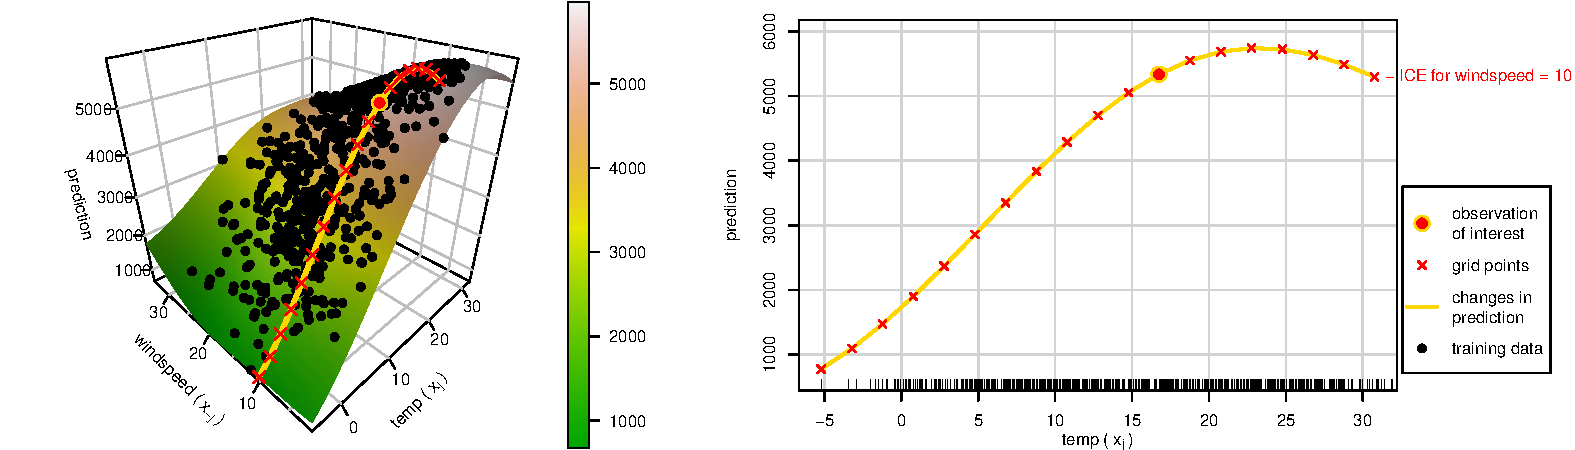
\includegraphics[width=0.95\textwidth, page = 1]{figure/ice_motivation_bike}

%$\Rightarrow$ Repeat for all observations and average the curves for global feature effect ($\leadsto$ PD plots)
\end{frame}



\begin{frame}{PD Plot - Global Feature Effects for ML Models}

\textbf{Question:} How do changes of feature values affect model prediction \textbf{on average}?

%\textbf{Idea:} 

\begin{itemize}
    \item \textbf{PD function}: Integrate out effect of $X_{-j}$ to obtain marginal effect of feature $x_j$
    
    \medskip
    
    \centerline{$ \textstyle
    f_j^{PD}(\tilde x_j) = \E_{X_{-j}}[\hat f(\tilde x_j, X_{-j})] = \int \hat f(\tilde x_j, X_{-j}) d \mathbb{P}(X_{-j})
    $}
        %with $C = S^\complement$. 

    \smallskip
    
    \item \textbf{Estimate (MC integration):} Average ICE curves at grid points $\tilde x_j$
    
    \medskip
    
    \centerline{$ \textstyle
    \hat f_j^{PD}(\tilde x_j) = \frac{1}{n} \sum_{i=1}^{n} \hat f(\tilde x_j, \xv_{-j}^{(i)})
    $}
\end{itemize}


\vfill
\centering
\includegraphics[width=0.95\textwidth, page = 2]{figure/ice_motivation_bike}

%Aggregates to Global PD
%point-wise average of ICE
%Extrapolation?
\end{frame}



\begin{frame}{Feature Interactions}

\textbf{Hooker (2004, 2007):} Functional ANOVA decomposition of a (prediction) function% into main and higher-order (interaction) effects

\begin{center}
    $\textstyle
\hat{f}(\mathbf{x}) = g_0 + 
\underbrace{\textstyle\sum_{j=1}^{p} {{g_j(x_j)}}}_{\text{{main effect}}} + 
\underbrace{\textstyle\sum_{j \neq k} {\textcolor{blue}{g_{j,k}(x_j, x_k)}}}_{\text{\textcolor{blue}{two-way interaction effect}}} + 
\cdots + 
\underbrace{{\textcolor{blue}{g_{1,2,\ldots,p}(\mathbf{x})}}}_{\text{\textcolor{blue}{p-way interaction effect}}}
$
\end{center}

%A function $f(\xv)$ is said to exhibit an interaction between two of its variables $x_j$ and $x_k$ if the difference in the value of $f(\xv)$ as a result of changing the value of $x_j$ depends on the value of $x_k$. For numeric variables, this can be expressed as
\textbf{Friedman and Popescu (2008):} %From functional ANOVA decomposition it follows
%A function $f(\xv)$ contains an interaction between $x_j$ and $x_k$ if a change in $f(\xv)$-values due to variations in $x_j$ also depend on $x_k$, i.e.: %, for numeric features:

%\medskip

%\centerline{$\mathbb{E} \left[ \tfrac{\partial^2 f(\xv)}{\partial x_j \partial x_k} \right]^2 > 0$}

%\medskip
\begin{itemize}
%is a sum of two functions, each independent of $x_j$, $x_k$:
% $f_{-j}$ and $f_{-k}$ that do not depend on $x_j$ and $x_k$, respectively:
    \item[$\Rightarrow$] If $x_j$ and $\xv_{-j}$ do not interact, we can decompose $f(\xv) = g_{j}(x_{j}) + g_{-j}(\xv_{-j})$
    \item[$\Rightarrow$] If $x_j$ and $x_k$ do not interact, we can decompose $f(\xv) = g_{-j}(\xv_{-j}) + g_{-k}(\xv_{-k})$
    %\item<3>[$\Rightarrow$] $\highlight{f(\xv) - g_{j}(x_{j}) - g_{-j}(\xv_{-j})} = 0$ %if there are no interactions between feature $j$ and any other feature $-j$
\end{itemize}


%\medskip

%\centerline{$f(\xv) = f_{-j}(x_1, \ldots, x_{j-1}, x_{j+1}, \ldots, x_p) + f_{-k}(x_1, \ldots, x_{k-1}, x_{k+1}, \ldots, x_p)$}


\only<1>{
{
\textbf{Example:} Not additively separable

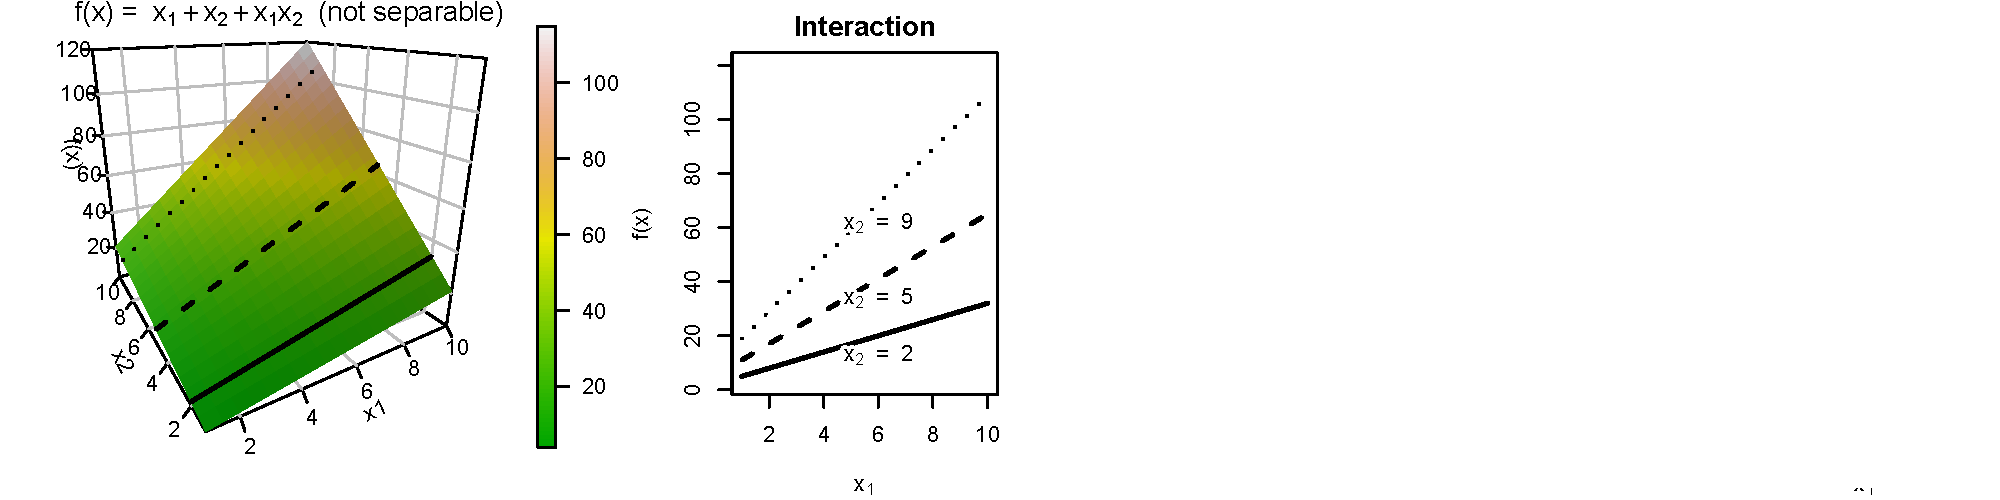
\includegraphics[width = 0.9\textwidth]{figure/interaction_separable_3}}
}
\only<2>{\textbf{Example:} Separable: {\footnotesize $f(\xv) = x_1 + x_2 + \log(x_1 \cdot x_2)
 	       = x_1 + \log(x_1) + x_2 + \log(x_2) = g_1(x_1) + g_2(x_2)$}
% \begin{itemize}
%     \item Not separable: $f(\xv) = x_1 + x_2 + x_1 \cdot x_2$
%     \item Separable: {\small $f(\xv) = x_1 + x_2 + \log(x_1 \cdot x_2)
% 	       = x_1 + \log(x_1) + x_2 + \log(x_2) = g_1(x_1) + g_2(x_2)$}
% \end{itemize}

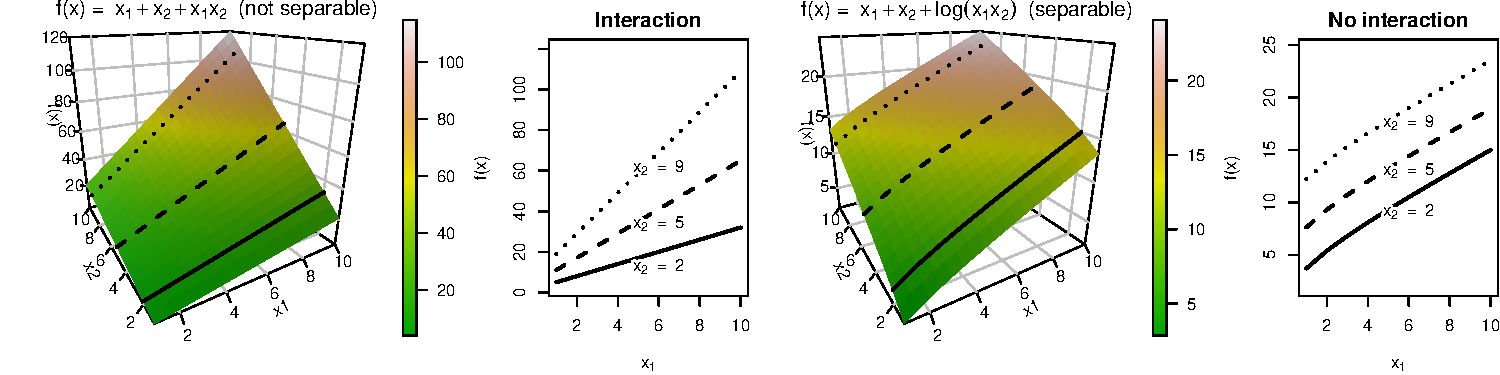
\includegraphics[width = 0.9\textwidth]{figure/interaction_separable_2}
%\pause\color{red}
%$\Rightarrow$ \textbf{Different shapes of ICE curves indicate interactions}
% ICE curves can be used to identify potential interactions (different shapes)
}
% \only<3>{

% \textbf{H-statistic:}

% The more $f^{PD,c}_{j}(x_j) + f^{PD,c}_{k}(x_k)$ deviates from $f_{j,k}^{PD,c}(\xv_{j,k})$, the stronger they interact:
% %The stronger a pair-wise interaction effect, the more the sum of $f^{PD,c}_{j}(\xv_j)$ and $f^{PD,c}_{k}(\xv_k)$ will deviate from $f_{j,k}^{PD,c}(\xv_{j,k})$

% \medskip

% \centerline{$ \displaystyle
%     \mathcal{\hat H}_{j,k}^2 = \frac{\sum\nolimits_{i=1}^n \left( 
%     \hat f_{j,k}^{PD,c}(\xi_{j,k}) -  \left(\hat f_{j}^{PD,c}(x_j) + \hat f_{k}^{PD,c}(x_k) \right)
%     \right)^2}{\sum_{i=1}^n \left( \hat f_{j,k}^{PD,c}(\xi_{j,k}) \right)^2 }, \text{ where}$}

% $\fh_{S}^{PD,c}$ is the mean-centered PD function with $\E \left( \fh_{S}^{PD,c}(X_S) \right) = 0$ for any set $S \subset \{1, \dots, p\}$

% % Measures how much a feature $j$ interacts with any other feature:

% % \medskip

% % \centerline{$ \displaystyle H^2_{j} = \frac{\sum_{i=1}^n\left[\highlight{\fh^c(\xv^{(i)}) - \fh_{j}^{PD,c}(x_j^{(i)}) - \fh_{-j}^{PD,c}(\xv_{-j}^{(i)}) } \right]^2}{\sum_{i=1}^n \left[\fh^c(\xv^{(i)}) \right]^2}, \text{ where}$}

% % \begin{itemize}
% %     \item $\fh^c$: mean-centered prediction function with $\E \left(\fh^c (X)\right) = 0$
% %     \item $\fh_{S}^{PD,c}$ mean-centered PD function with $\E \left( \fh_{S}^{PD,c}(X_S) \right) = 0$ for any set $S \subset \{1, \dots, p\}$
% % \end{itemize}


% }
\end{frame}





\begin{frame}{REPID: Regional Effect Plots \citebutton{Herbinger et al. (2022)}{https://proceedings.mlr.press/v151/herbinger22a.html}}

\textbf{Recall:} Different shapes of ICE curves indicate interactions (we want to ignore vertical shifts)\\
$\Rightarrow$ Focus on shape differences of {\color{cice}\bfseries mean-centered ICE curves}.
    
%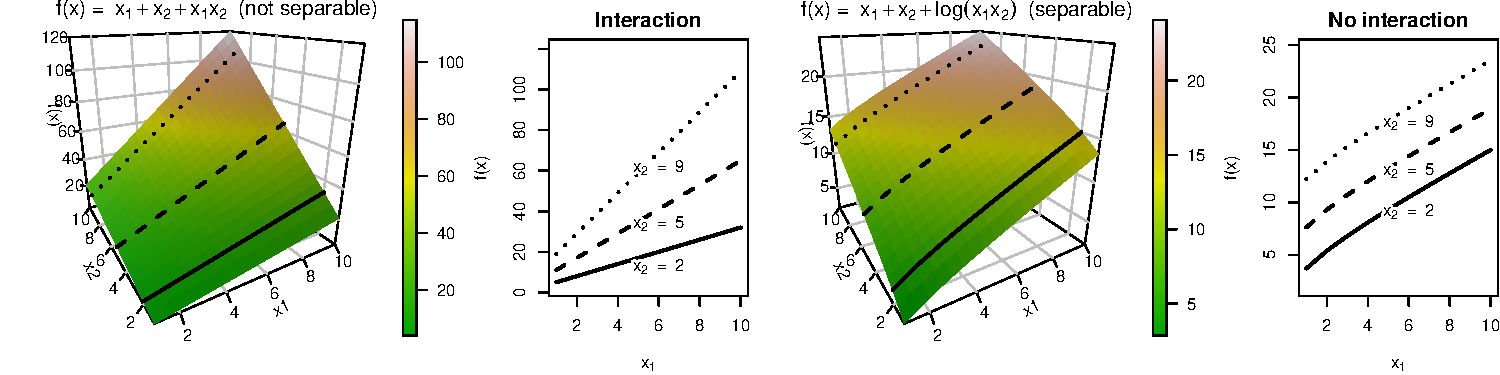
\includegraphics[width = 0.8\textwidth, trim={0cm 0cm 0cm 0cm}, clip]{figure/interaction_separable_2}

The mean-centered ICE curve for obs. $\xv$ evaluated at $m$ grid points $\tilde x_j^{(1)}, \dots, \tilde x_j^{(m)}$ is:

{\color{cice}
\centerline{$\hat f^c(\tilde x_j, \xv_{-j}) = \hat{f}(\tilde x_j, \xv_{-j}) - \frac{1}{m} \sum\nolimits_{k=1}^m \hat{f}(\tilde x_j^{(k)}, \xv_{-j})$}}
 %and $g \in \{1,...,G\}$

\begin{columns}
    \begin{column}{0.39\textwidth}
        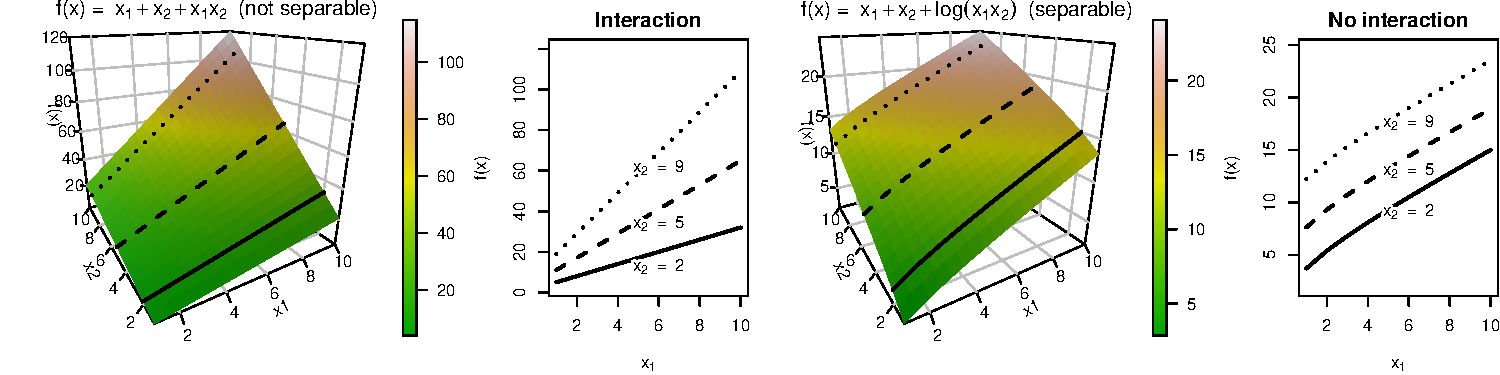
\includegraphics[width = \textwidth, trim={13cm 0cm 0cm 0cm}, clip]{figure/interaction_separable_2}
    \end{column}
    \begin{column}{0.61\textwidth}
        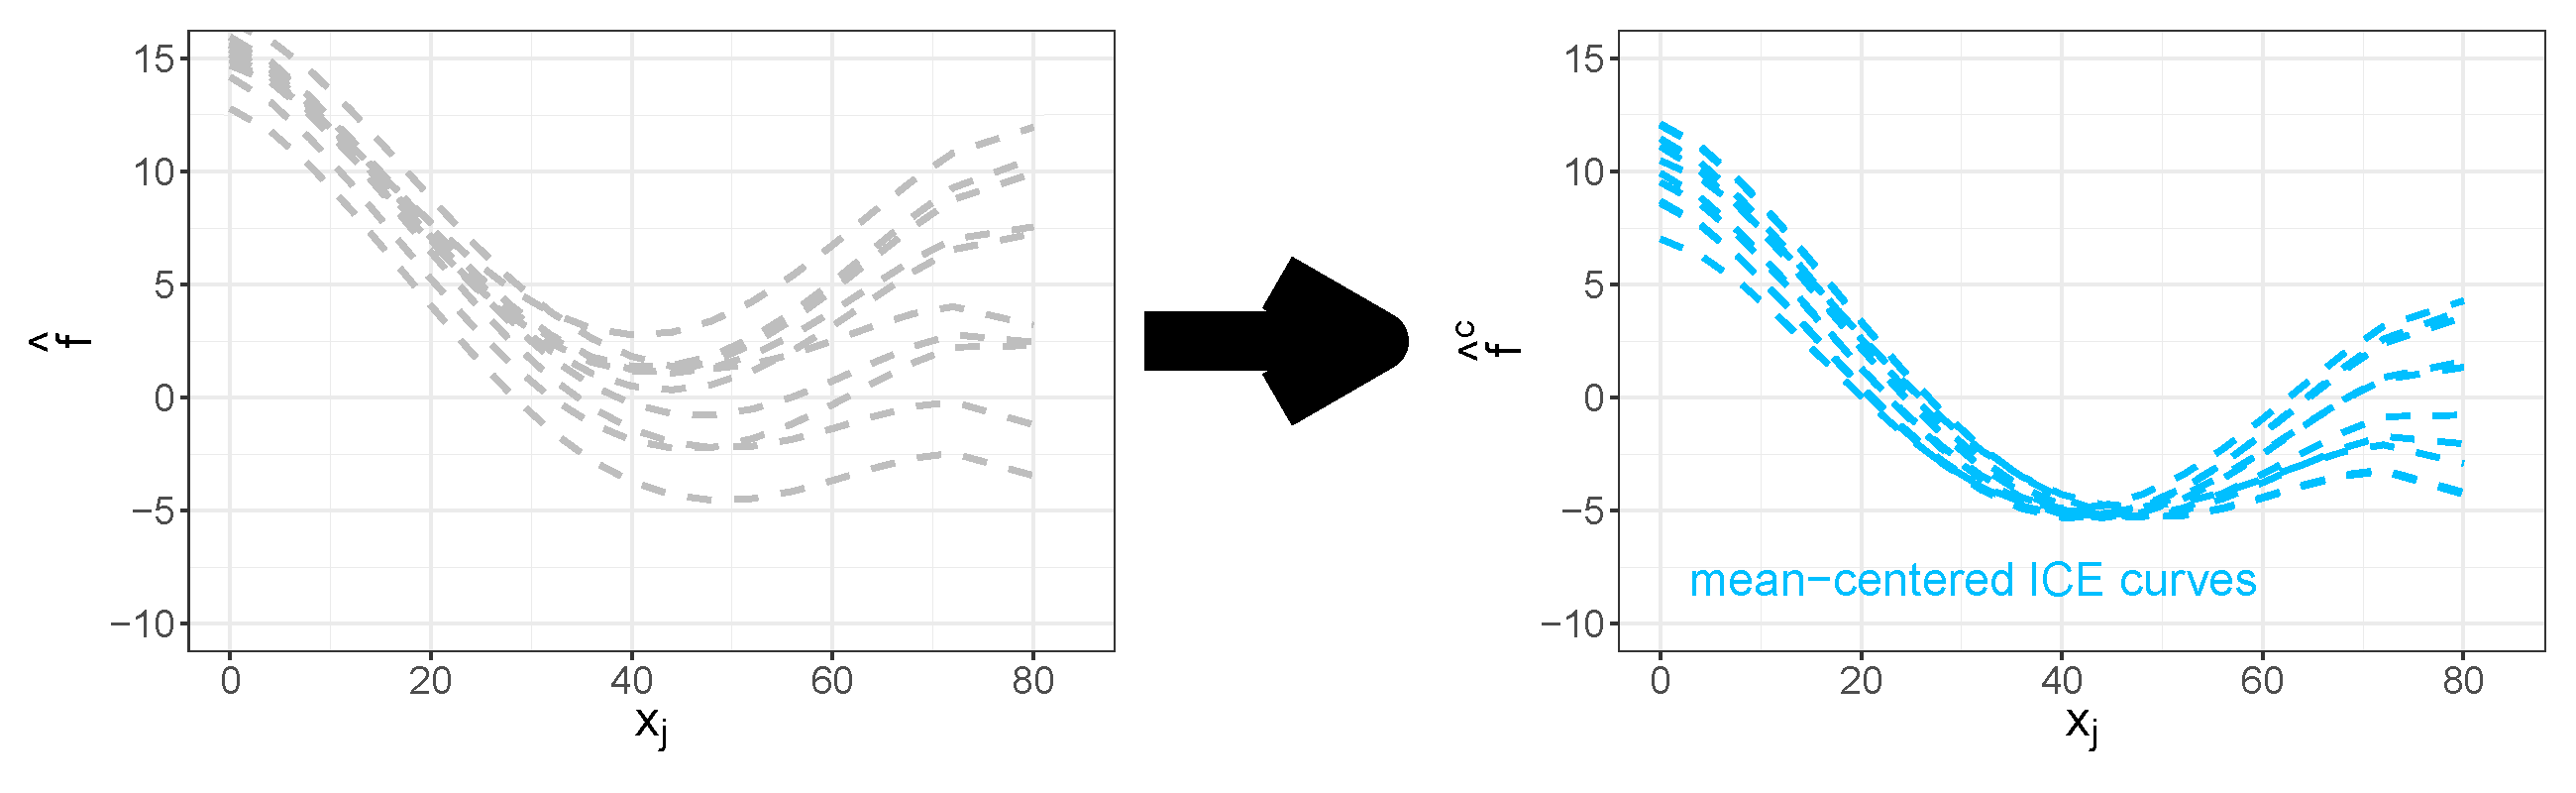
\includegraphics[width = \textwidth]{figure/ice_rep_distance0.png} 
    \end{column}
\end{columns}

%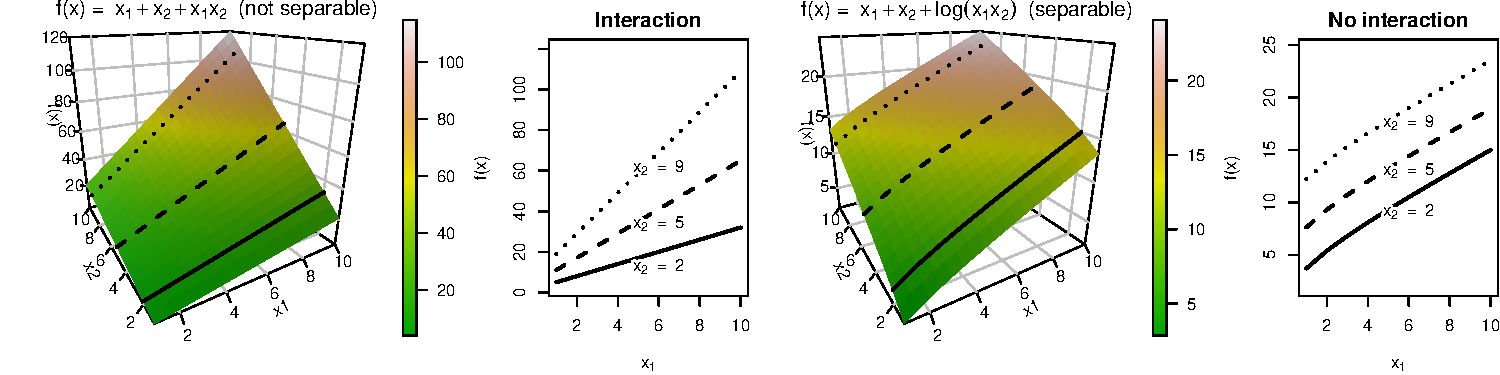
\includegraphics[width = 0.3\textwidth, trim={13cm 0cm 0cm 0cm}, clip]{figure/interaction_separable_2}
\end{frame}

\begin{frame}{Regional Effect Plots - Intuition}

\begin{columns}[T, totalwidth=\textwidth]
    \begin{column}{0.6\textwidth}
 Define risk as the L2 loss of mean-centered ICE curves:
$$\textstyle
    \mathcal{R}\left(\mathcal{N}\right) =
    \sum\limits_{\xv \in \mathcal{N}} 
     \sum\limits_{k = 1}^m
     (\underbrace{{\color{cice}\hat f^{c}(\tilde x_j^{(k)}, \xv_{-j})} - \color{rep}\hat f_{j|\mathcal{N}}^{PD,c} (\tilde x_j^{(k)})}_\text{$\color{orange}{d_k}$})^2
    %\mathcal{L}\left(\xv_j, i\right)
    $$
with the average feature effect in %region with associated index set 
region $\mathcal{N} \subseteq \Xspace$:

\medskip

{\color{rep}
\centerline{$ \displaystyle    \hat f_{j|\mathcal{N}}^{PD,c}(\tilde x_j) = \frac{1}{|\mathcal{N}|} \sum_{\xv \in \mathcal{N}} \hat f^c(\tilde x_j, \xv_{-j})$}}
    \end{column}
    \begin{column}{0.39\textwidth}
            \centering
    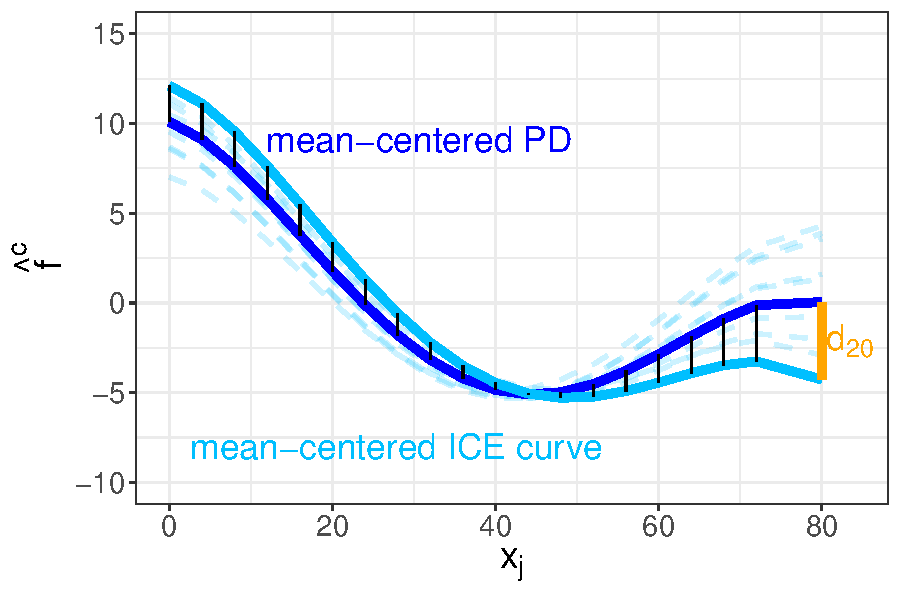
\includegraphics[width = \textwidth]{figure/ice_rep_distance2.pdf}
    \end{column}
\end{columns}
%\medskip
\begin{itemize}
    \item[$\Rightarrow$] Measures interaction-related heterogeneity (variance) ICE curves in region $\mathcal{N}$
    \item[$\Rightarrow$] Recursive partitioning (as in CART): Find the best feature-split combination that minimizes
    
\medskip

\centerline{$\mathcal{R}\left(\mathcal{N}_{left}\right) + \mathcal{R}\left(\mathcal{N}_{right}\right)$}
\end{itemize}

      \begin{columns}[c, totalwidth=\textwidth]
        \begin{column}{0.4\textwidth}
    \begin{itemize}
        \item $\mathcal{N}_{left} = \{\xv \in \mathcal{N}|x_z \leq t\}$
        \item $\mathcal{N}_{right} = \{\xv \in \mathcal{N}|x_z > t\}$
        \item Split point $t$ for feature $x_z, z \in -j$
    \end{itemize}
        \end{column}
          \begin{column}{0.59\textwidth}
          \centering
          \textbf{Intuition:} Is another feature $x_z$ \\responsible for the heterogeneity?
        \end{column}
    \end{columns}
        %\item loss $\mathcal{L}$ for $i$-th ICE curve based on a grid of size $m$
        %\item aggregate over all ICEs within region $\mathcal{N}$
    %\end{itemize}
%\footnote[frame]{\textbf{AISTATS 2022:} \textit{REPID - Regional Effect Plots with implicit Interaction Detection}}
\end{frame}




\begin{frame}{Regional Effect Plots - Example}

   
%\textbf{How can we use ICE curves to find regions with representative PDPs?}
%\vspace*{0.3cm}

\begin{columns}[T, totalwidth = \linewidth]
    \begin{column}{0.42\textwidth}


\textbf{Example:}
%$X_1, X_2 \sim \mathcal{U}(-1,1), X_3, X_5 \sim \mathcal{B}(n, 0.5), X_4 \sim \mathcal{B}(n, 0.7), X_6 \sim \mathcal{N}(1,5)$ (all iid)\\
$X_1, X_2, X_6 \sim \mathcal{U}(-1,1)$, 
$X_3, X_4, X_5 \sim \mathcal{B}(n, 0.5)$ (all iid)\\

%$\leadsto$ True relationship: $f(X) = 0.2 X_1 - 8 X_2 + \color{YellowGreen}{8 X_2  \mathbbm{1}_{(X_1 > 0)}} \color{black}+ \color{ForestGreen}{16 X_2  \mathbbm{1}_{(X_3 = 0)}} \color{black}+ \epsilon, \; \epsilon \sim \mathcal{N}(0,1)$\\

$\leadsto$ Model: Random forest

        \begin{itemize}
  %\setlength{\itemindent}{0em}
\item \textbf{Problem:} 
\begin{itemize}
    \item \only<1>{PD curve of $\highlight{X_2}$ is misleading due to interactions $\leadsto$ ICE}
    \only<2->{PD curve of $X_2$ is misleading due to interactions $\leadsto$ ICE}
    \item ICE curves do not identify the interacting features
\end{itemize}

\item<2-> \textbf{Idea:} Find regions where variance of ICE curves is minimized by recursive partitioning the feature space w.r.t. all other features $-j$\\
%Find regions with similar ICE curves and aggregate them to regional effects\\
%\item 
%$\leadsto$ REP more representative due to less interactions  
   %\item[$\leadsto$]\textbf{Idea} Recursively partition feature space w.r.t. $-j$ such that distance of ICE curves to REP is small}
\item<3-> {\color{rep}\textbf{Regional effect}} (blue curves)   $\hat = $ Estimate PD curve in each region

 % \centerline{$ \textstyle    \hat f_{j|\mathcal{N}_g}^{PD}(\tilde x_j) = \frac{1}{|\mathcal{N}_g|} \sum_{i \in \mathcal{N}_g} \hat f(\tilde x_j, \xv_{-j}^{(i)})$}
\end{itemize}


   
    \end{column}
    \begin{column}{0.55\textwidth}
    \small
    \only<1>{\centerline{
    $f(X) = 0.2 X_1 \highlight{- 8 X_2 + {8 X_2  \mathbbm{1}_{(X_1 > 0)}}+ {16 X_2  \mathbbm{1}_{(X_3 = 0)}}} + \epsilon $}}
    \only<2>{\centerline{
    $f(X) = 0.2 X_1 - 8 X_2 + {8 X_2  \mathbbm{1}_{(X_1 > 0)}} + \highlightFG{16 X_2  \mathbbm{1}_{(X_3 = 0)}} \color{black}+ \epsilon $}}
    \only<3>{\centerline{
    $f(X) = 0.2 X_1 - 8 X_2 + \highlightYG{8 X_2  \mathbbm{1}_{(X_1 > 0)}} \color{black}+ \highlightFG{16 X_2  \mathbbm{1}_{(X_3 = 0)}} \color{black}+ \epsilon $}}
    %$, \; \epsilon \sim \mathcal{N}(0,1)$
\only<1>{
    \centering
      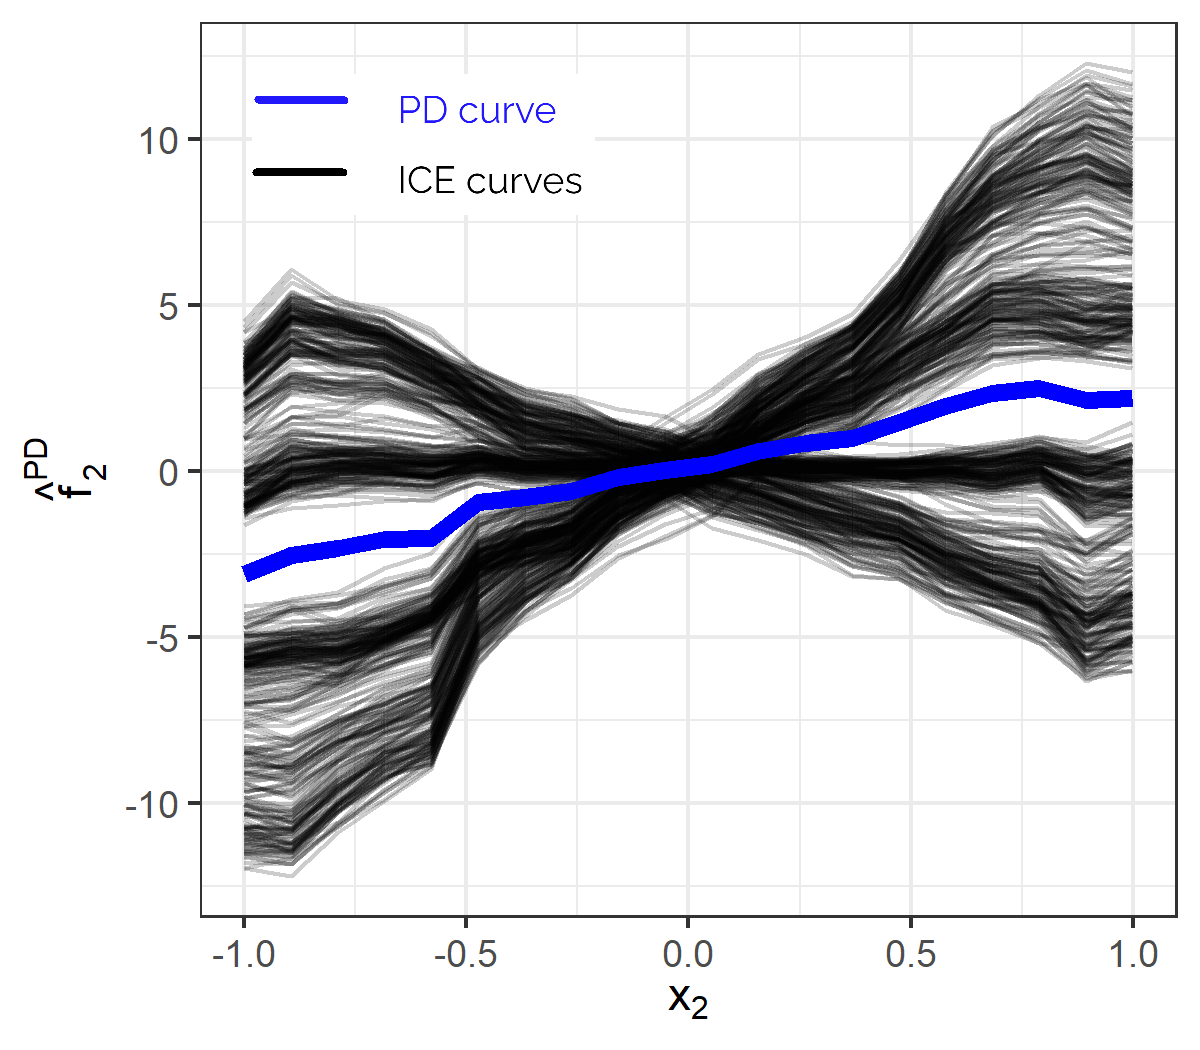
\includegraphics[width=0.82\textwidth]{figure/sim1_allcurves.png} 
}
\only<2->{
\centering
     %\begin{minipage}[t]{.5\textwidth}
     \hspace{-20pt}
     \includegraphics<2>[width=0.5\textwidth]{figure/sim1_allcurves.png}
     
     \only<2>{
           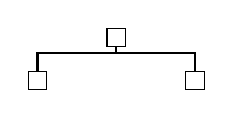
\begin{tikzpicture}
      \usetikzlibrary{arrows}
        \usetikzlibrary{shapes}
         \tikzset{treenode/.style={draw}}
         \tikzset{line/.style={draw, thick}}
     % Nodes
    \node [treenode] (a0) {}; [below=1pt,at=(10,0)]  {};% Top node
    \node [treenode, below=0.3cm of a0, xshift=-1.0cm] (a1) {}; % Bottom left node
    \node [treenode, below=0.3cm of a0, xshift=1.0cm] (a2) {}; % Bottom right node

    % Lines
    \draw [thick] (a0) -- ++(0, -0.2cm) -| (a1);
    \draw [thick] (a0) -- ++(0, -0.2cm) -| (a2);
      \end{tikzpicture}
     }
     
      %\fcolorbox{ForestGreen}{white}     {
      \highlightFG{
      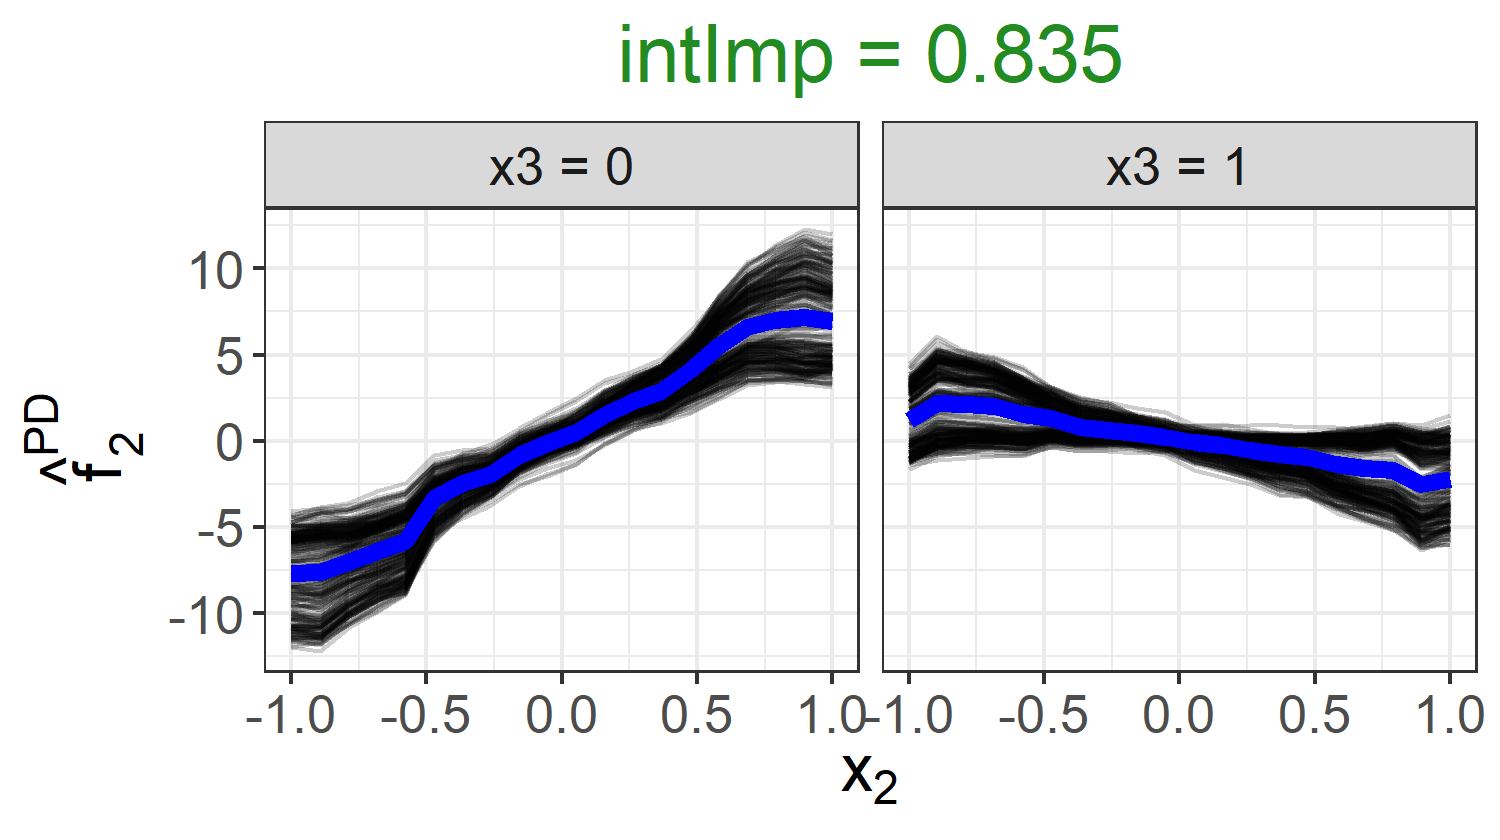
\includegraphics[width=0.6\textwidth, trim = 0 0 0 25, clip]{figure/sim1_dt_split1.png}
      }
      %}
}
\only<3->{
      \scalebox{1}{
      \hspace{15pt} 
      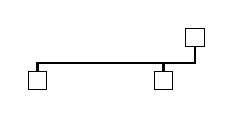
\begin{tikzpicture}
      \usetikzlibrary{arrows}
        \usetikzlibrary{shapes}
         \tikzset{treenode/.style={draw}}
         \tikzset{line/.style={draw, thick}}
        \node [treenode](a0) {} ; [below=1pt,at=(4,0)]  {};
         \node [treenode, below=0.3cm, at=(a0.south), xshift=-2.0cm]  (a1) {};
         \node [treenode, below=0.3cm, at=(a0.south), xshift=-0.4cm]  (a2) {};
         \path [line] (a0.south) -- + (0,-0.2cm) -| (a1.north) node [midway, above] {};
         \path [line] (a0.south) -- +(0,-0.2cm) -|  (a2.north) node [midway, above] {};
      \end{tikzpicture}
      \hspace{35pt}
      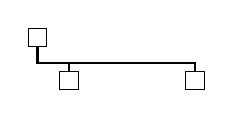
\begin{tikzpicture}
      \usetikzlibrary{arrows}
        \usetikzlibrary{shapes}
         \tikzset{treenode/.style={draw}}
         \tikzset{line/.style={draw, thick}}
        \node [treenode] (a01) {};[below=5pt,at=(node1.south) , xshift=3.5cm]
         \node [treenode, below=0.3cm, at=(a01.south), xshift=0.4cm]  (a1) {};
         \node [treenode, below=0.3cm, at=(a01.south), xshift=2.0cm]  (a2) {};
         \path [line] (a01.south) -- + (0,-0.2cm) -| (a1.north) node [midway, above] {};
         \path [line] (a01.south) -- +(0,-0.2cm) -|  (a2.north) node [midway, above] {};
      \end{tikzpicture}
      }
    %\fcolorbox{YellowGreen}{white}{
    \highlightYG{
    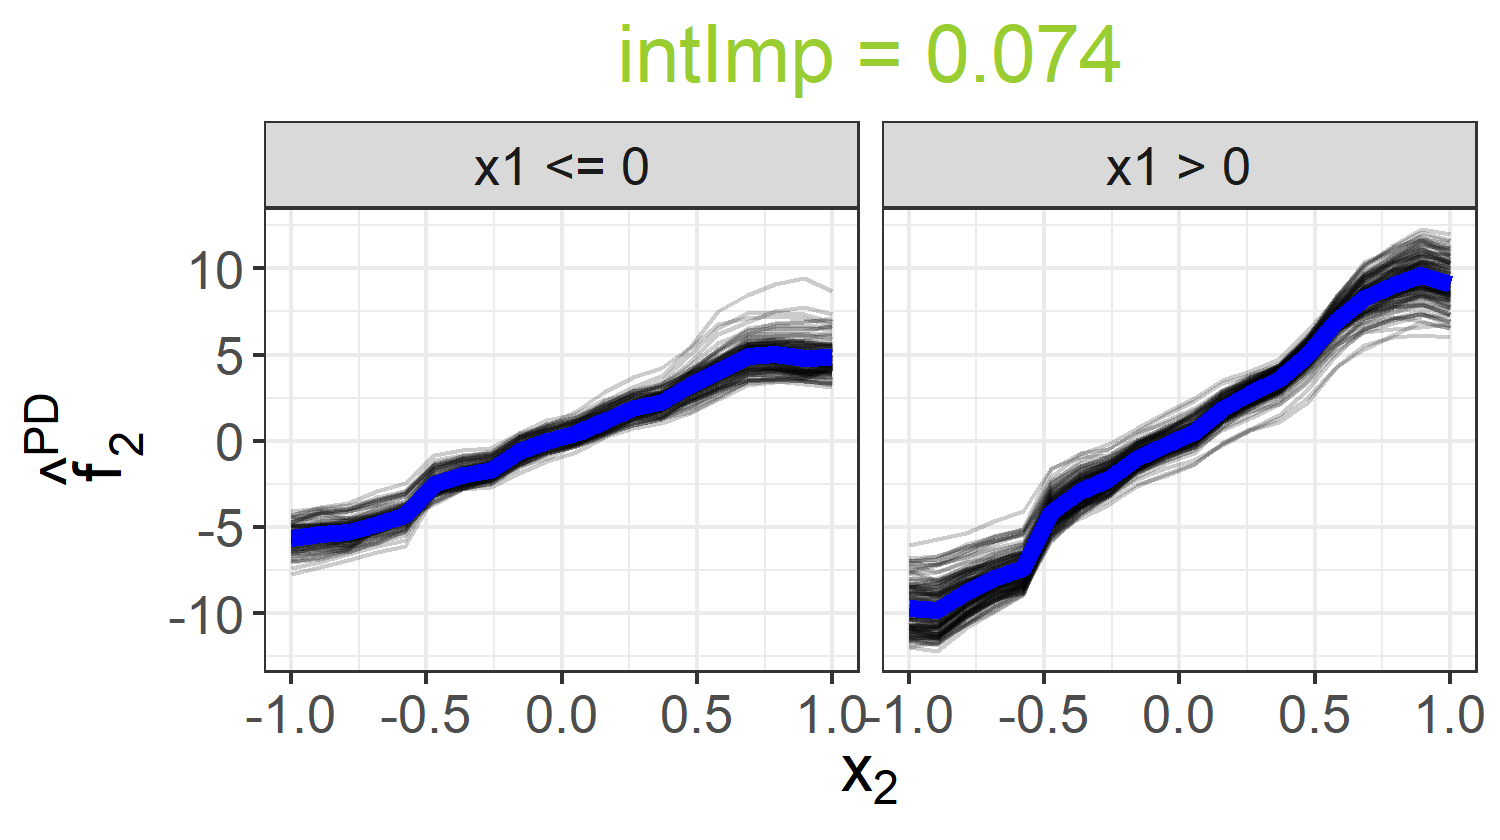
\includegraphics[width=0.52\textwidth, trim = 0 0 0 25, clip]{figure/sim1_dt_split2_1.png}
    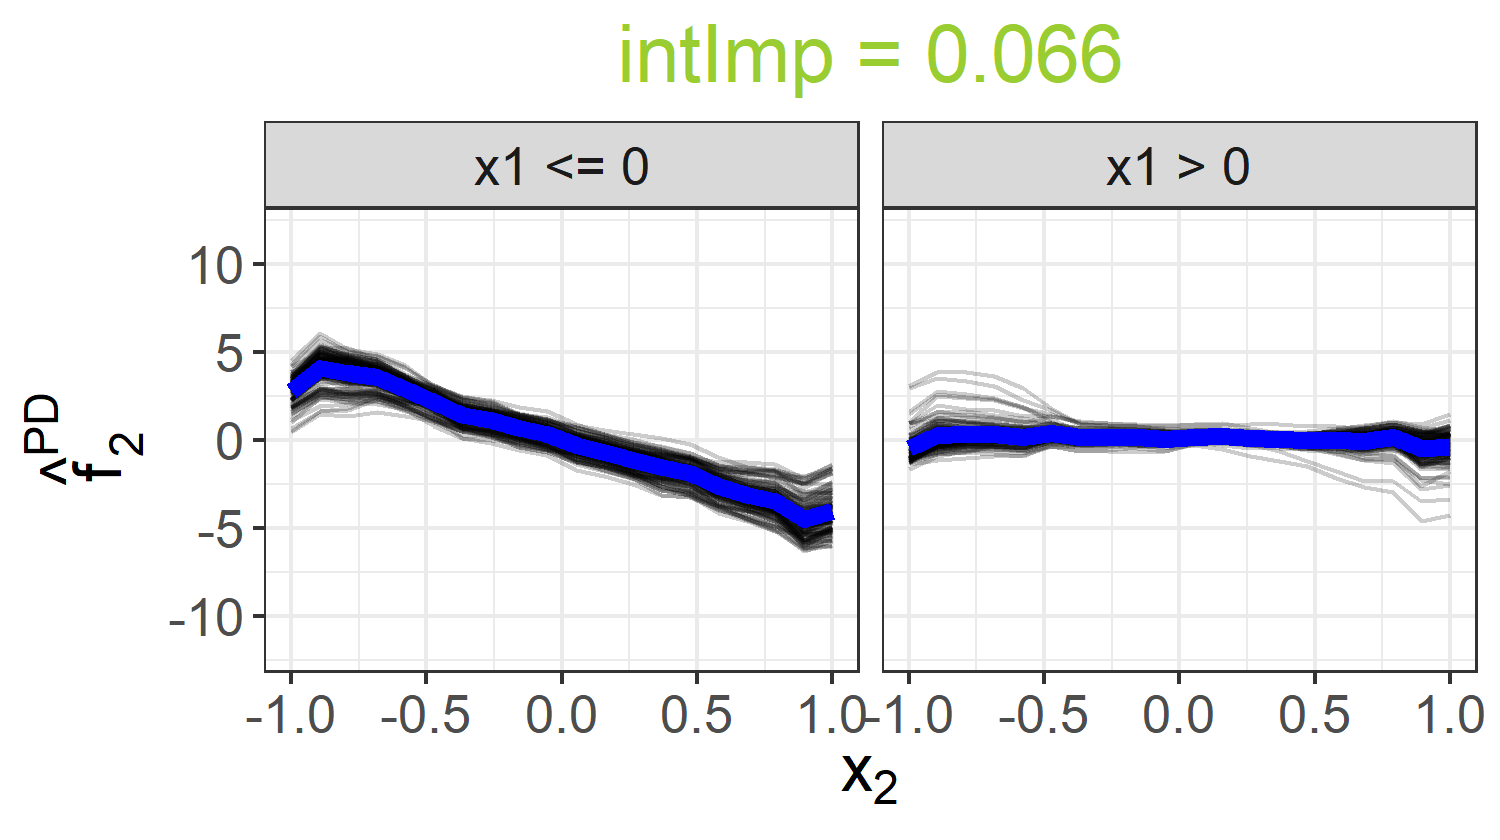
\includegraphics[width=0.46\textwidth, trim = 40 0 0 25, clip]{figure/sim1_dt_split2_2.png}
    }
    %\vspace{.2in}
    %\caption{ICE curves for $\xv_2$ are grouped by REPID and REPs (blue) are illustrated. %The first split divides the ICE curves depending on $x_3$. The second level divides the ICE curves of each child node again into two sub-regions with respect to $x_1$.
    %}
    %\label{fig:sim1_dt}
     %\end{minipage} 

     \begin{columns}[T, totalwidth = \linewidth]
     %\footnotesize
            \begin{column}{0.1\linewidth}
            \centering
             $\hat{f}_2^{PD}(X_2)$ %, X_1 > 0 \land X_3 = 0\)\\
         \end{column}
         \begin{column}{0.18\linewidth}
         \centering
             $\approx 8X_2$ %, X_1 > 0 \land X_3 = 0\)\\
         \end{column}
        \begin{column}{0.2\linewidth}
\centering
            $\approx 16X_2$ %, X_1 \leq 0 \land X_3 = 0\)
         \end{column}
        \begin{column}{0.2\linewidth}
        \centering
            $ \approx -8X_2$ %, X_1 \leq 0 \land X_3 \neq 0\)
         \end{column}        
         \begin{column}{0.2\linewidth}
         \centering
             $\approx 0$%, X_1 > 0 \land X_3 \neq 0\)\\
         \end{column}
     \end{columns}
     \medskip
     $\Rightarrow$ Additive decomposition of global feature effect
     %$f_2(X_2) \approx \sum_{i: \textit{terminal node indices}} g_i(X_2) \mathbbm{1}_{(X \in \mathcal{N}_i)}$
}


    \end{column}

\end{columns}

% \begin{minipage}[htb]{0.48\linewidth}
% \begin{itemize}

% \item \textbf{Problem:} PD plot (average of ICE) misleading

% \item \textbf{Idea:} Find regions where ICE curves are similar in their shape\\
% $\leadsto$ These regions have little interactions 

%     %\item<1-2> Grouping homogeneous ICE curves reduces individual interaction effects
%     %\item<2> REP = group marginal effect for feature of interest $x_j$ in specific region
  
% \end{itemize}
% \end{minipage}
% \only<1>{
% \begin{minipage}[htb]{0.5\linewidth}
%     \centering
%      %\begin{minipage}[t]{.5\textwidth}
%       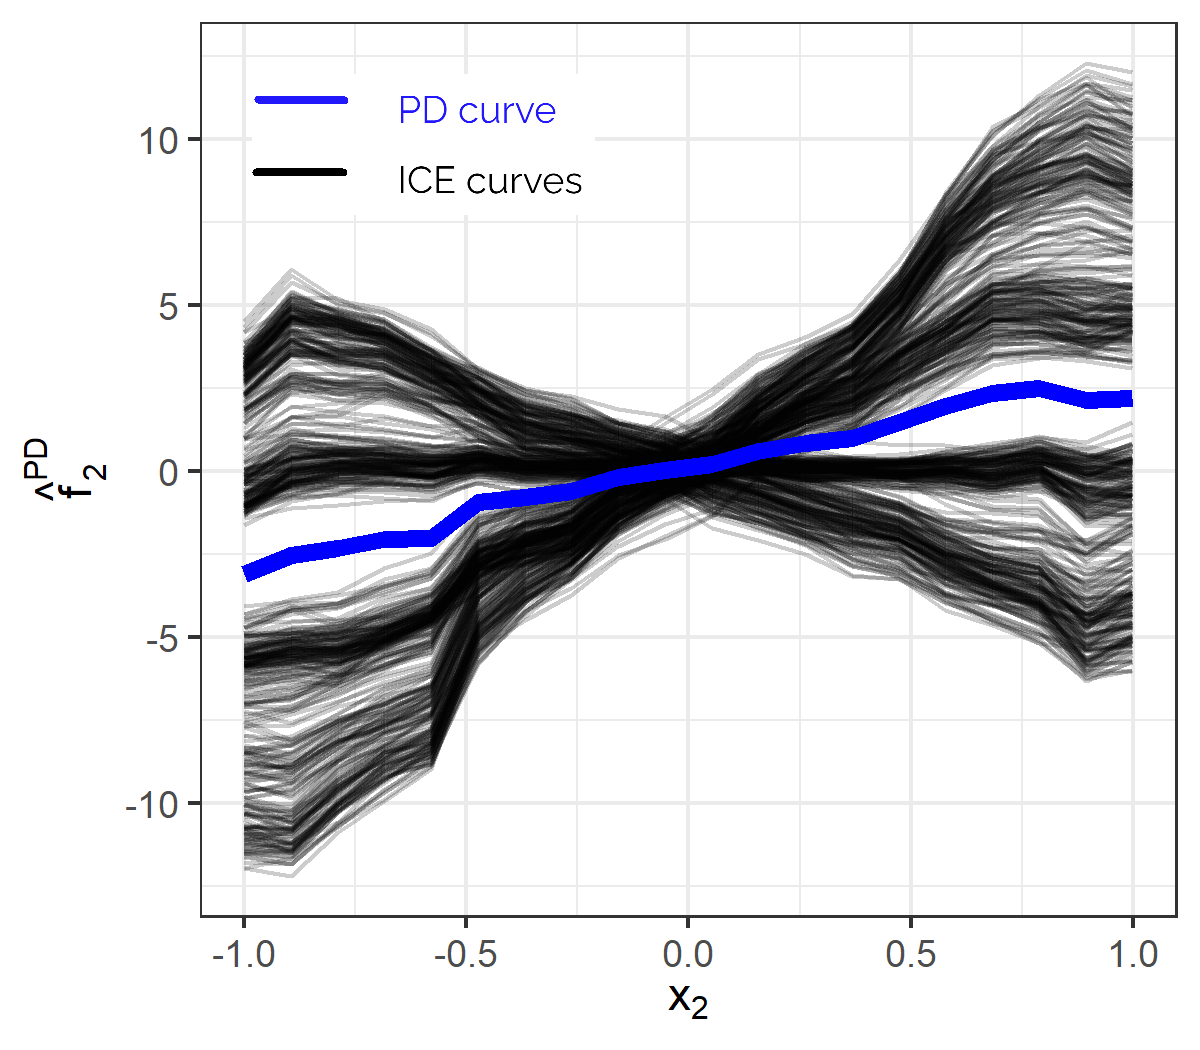
\includegraphics[width=0.9\textwidth]{figure/sim1_allcurves.png}
     
% \end{minipage}
% }
% \only<2>{
% \begin{minipage}[htb]{0.47\linewidth}
%     \centering
%      %\begin{minipage}[t]{.5\textwidth}
%       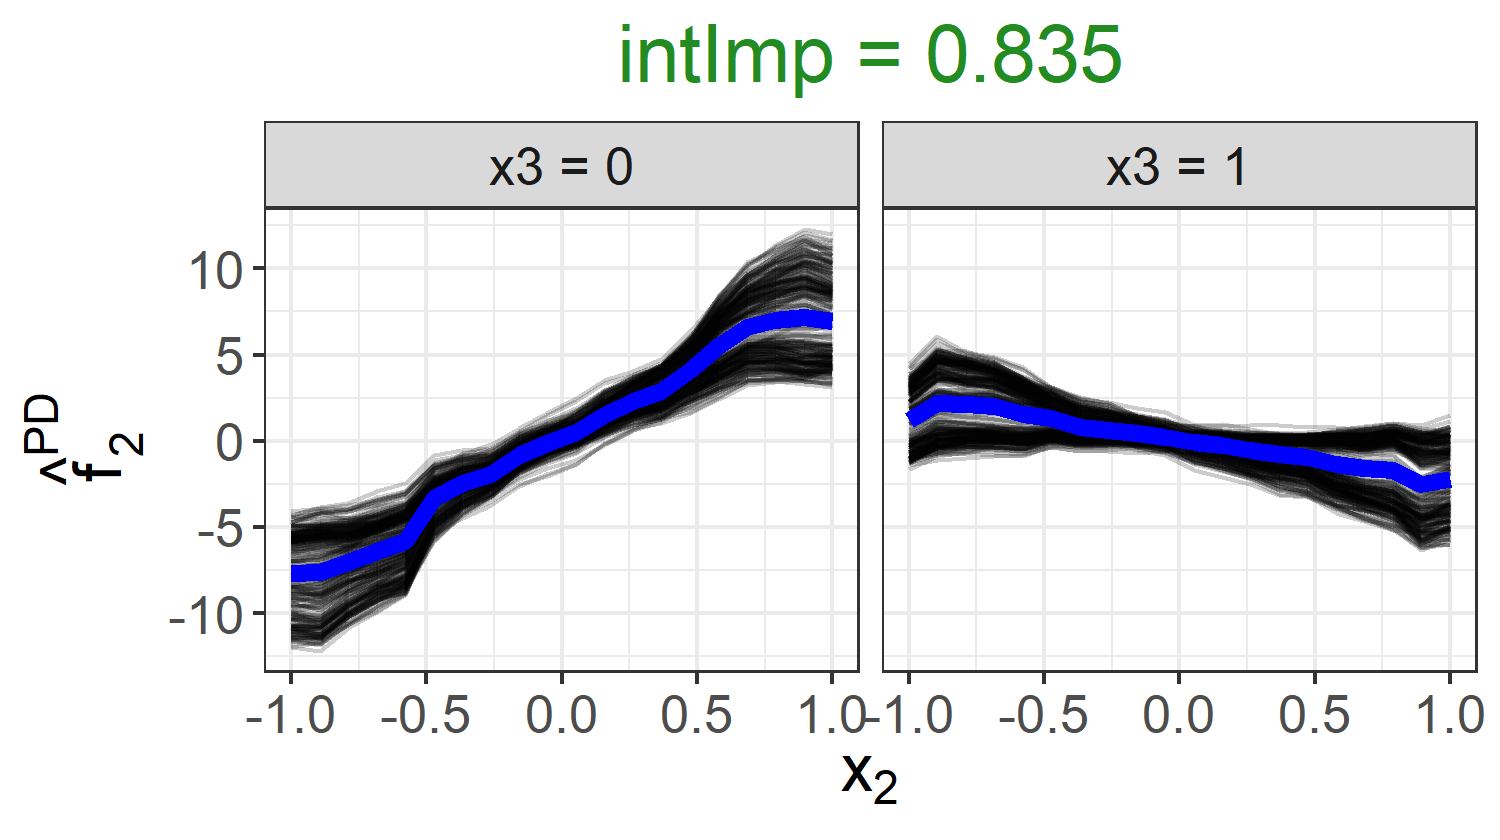
\includegraphics[width=0.49\textwidth]{figure/sim1_dt_split1.png}
%       \scalebox{1}{
%       \hspace{15pt} 
%       \begin{tikzpicture}
%       \usetikzlibrary{arrows}
%         \usetikzlibrary{shapes}
%          \tikzset{treenode/.style={draw}}
%          \tikzset{line/.style={draw, thick}}
%         \node [treenode](a0) {} ; [below=1pt,at=(4,0)]  {};
%          \node [treenode, below=0.3cm, at=(a0.south), xshift=-2.0cm]  (a1) {};
%          \node [treenode, below=0.3cm, at=(a0.south), xshift=-0.4cm]  (a2) {};
%          \path [line] (a0.south) -- + (0,-0.2cm) -| (a1.north) node [midway, above] {};
%          \path [line] (a0.south) -- +(0,-0.2cm) -|  (a2.north) node [midway, above] {};
%       \end{tikzpicture}
%       \hspace{35pt}
%       \begin{tikzpicture}
%       \usetikzlibrary{arrows}
%         \usetikzlibrary{shapes}
%          \tikzset{treenode/.style={draw}}
%          \tikzset{line/.style={draw, thick}}
%         \node [treenode] (a01) {};[below=5pt,at=(node1.south) , xshift=3.5cm]
%          \node [treenode, below=0.3cm, at=(a01.south), xshift=0.4cm]  (a1) {};
%          \node [treenode, below=0.3cm, at=(a01.south), xshift=2.0cm]  (a2) {};
%          \path [line] (a01.south) -- + (0,-0.2cm) -| (a1.north) node [midway, above] {};
%          \path [line] (a01.south) -- +(0,-0.2cm) -|  (a2.north) node [midway, above] {};
%       \end{tikzpicture}
%       }
%     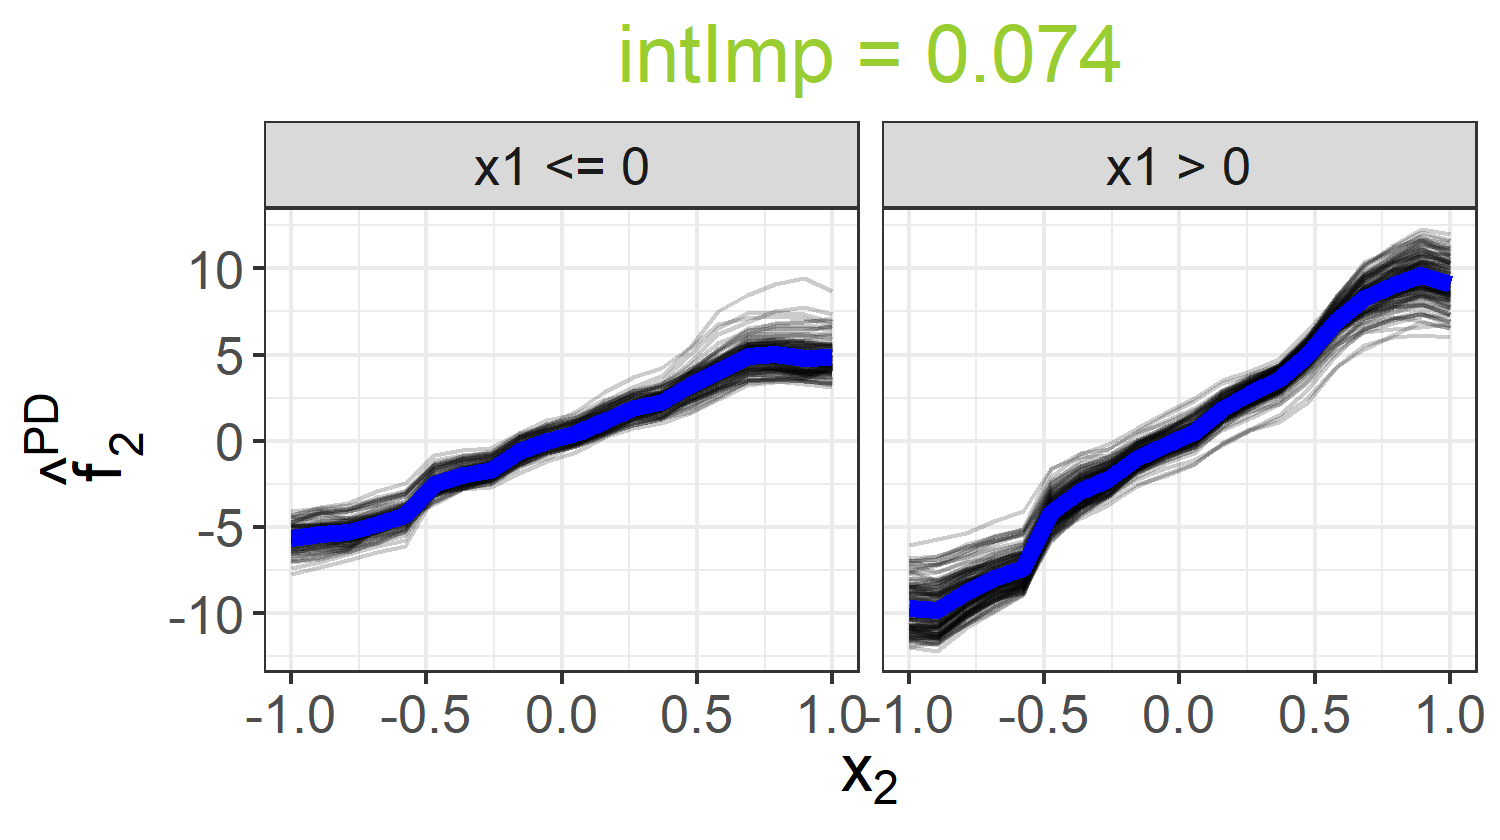
\includegraphics[width=0.49\textwidth]{figure/sim1_dt_split2_1.png}
%     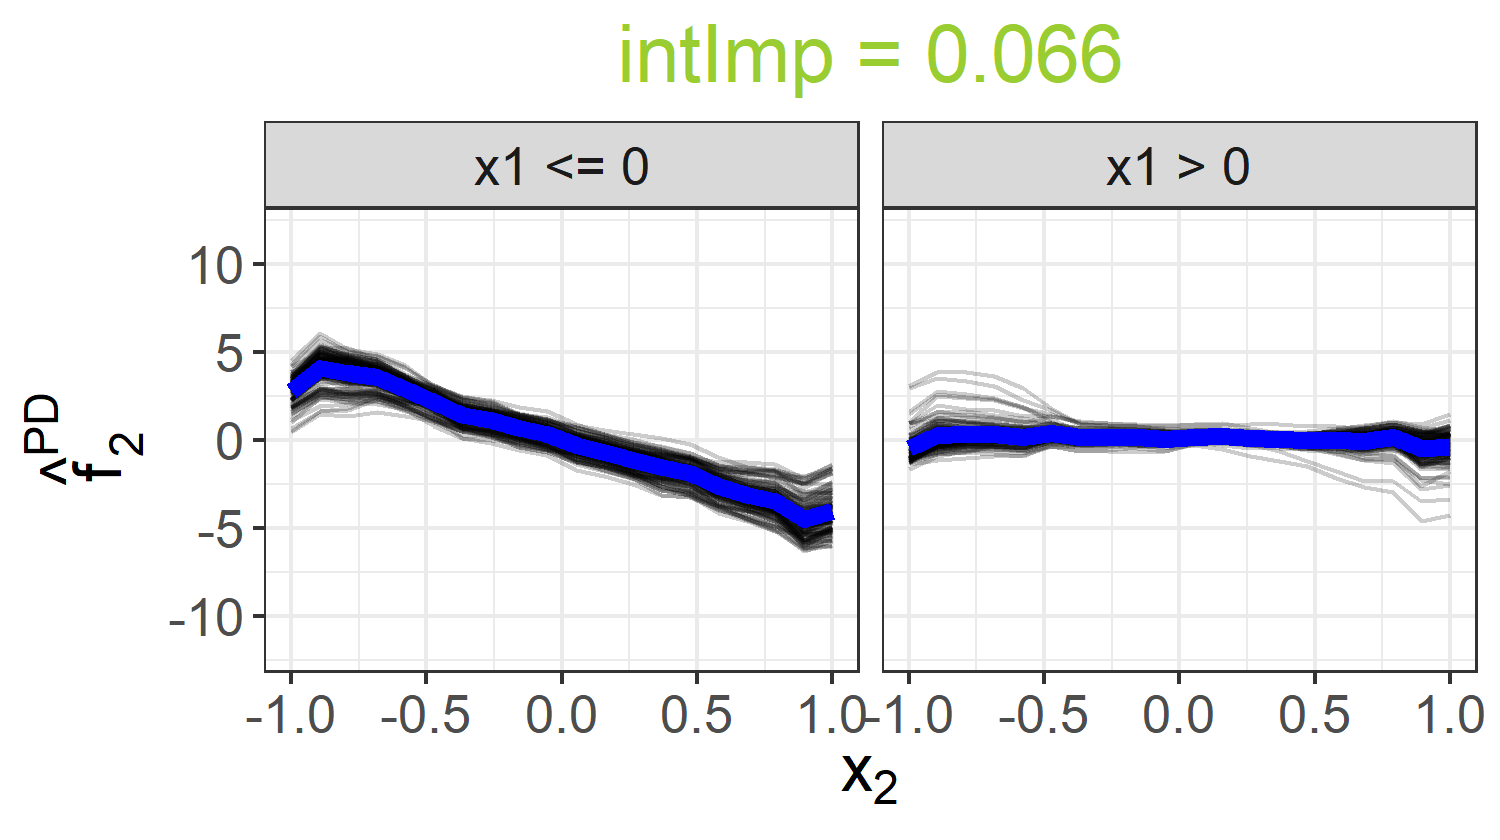
\includegraphics[width=0.49\textwidth]{figure/sim1_dt_split2_2.png}
%     \vspace{.2in}
%     %\caption{ICE curves for $\xv_2$ are grouped by REPID and REPs (blue) are illustrated. %The first split divides the ICE curves depending on $x_3$. The second level divides the ICE curves of each child node again into two sub-regions with respect to $x_1$.
%     %}
%     \label{fig:sim1_dt}
%      %\end{minipage} 
%\end{minipage}
%}


%\footnote[frame]{\textbf{AISTATS 2022:} \textit{REPID - Regional Effect Plots with implicit Interaction Detection}}

\end{frame}

%we want to split $\mathcal{N}$ in such a way that ICE curves within the obtained regions have a similar shape meaning that the distance of these ICE curves to the REP estimate (i.e., $\hat{f}^{PD}_{S|\mathcal{N}_g} (\xv_j):= \frac{1}{|\mathcal{N}_g|}\sum_{i \in \mathcal{N}_g} \hat{f}\left(\xv_j, \xv_C^{(i)}\right)$) is small.

% \begin{frame}{Regional Effect Plots - Functional Decomposition}

% What happened?

% \end{frame}




\begin{frame}{Interaction quantification}

\begin{columns}[T, totalwidth=\textwidth]
    \begin{column}{0.59\textwidth}

\textbf{On parent node level (for {\color{mygreen}$\mathcal{N}_{parent}$}):}
%Relative interaction importance for each parent node :
$$
   intImp({\color{mygreen}{\mathcal{N}_{parent}}}) = \frac{\mathcal{R}({\color{mygreen}\mathcal{N}_{parent}}) - (\mathcal{R}({\color{amber}\mathcal{N}_{left}}) + \mathcal{R}({\color{red}\mathcal{N}_{right}}))}{\mathcal{R}({\color{blue}\mathcal{N}})} 
$$
\textbf{Interpretation:}
Reduction of ICE curve variance after one split of $\mathcal{N}_{parent}$ into $\mathcal{N}_{left}$ and $\mathcal{N}_{right}$ 
relative to the ICE curve variance in the root node $\mathcal{N}$.

\medskip

\begin{center}
      \resizebox{0.5\linewidth}{!}{
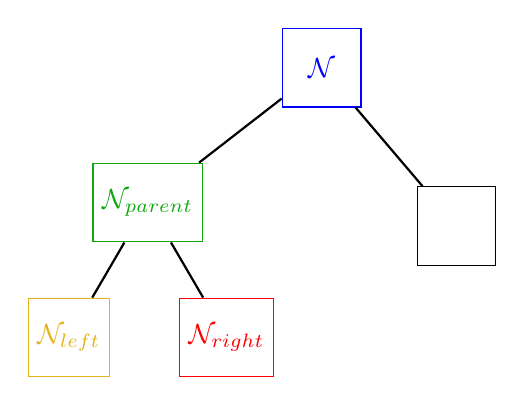
\begin{tikzpicture}
    \usetikzlibrary{arrows}
    \usetikzlibrary{shapes}

    % Define node styles
    \tikzset{
        treenode/.style={draw, rectangle, minimum size=1cm, text centered},
        N/.style={draw, rectangle, minimum size=1cm, text centered, color=blue, text=blue},
        Np/.style={draw, rectangle, minimum size=1cm, text centered, color=mygreen, text=mygreen},
        Nl/.style={draw, rectangle, minimum size=1cm, text centered, color=amber, text=amber},
        Nr/.style={draw, rectangle, minimum size=1cm, text centered, color=red, text=red}
    }

    % Nodes
    \node [N] (a0) {$\mathcal{N}$}; % Top node
    \node [treenode, below right=1cm and 0.7cm of a0] (a1) {}; % Bottom right node
    \node [Np, below left=0.7cm and 1cm of a0] (a2) {$\mathcal{N}_{parent}$}; % Bottom center node
    \node [Nl, below=0.7cm of a2, xshift=-1cm] (a3) {$\mathcal{N}_{left}$}; % Bottom left node
    \node [Nr, below=0.7cm of a2, xshift=1cm] (a4) {$\mathcal{N}_{right}$}; % Bottom right node from center

    % Lines
    \draw [thick] (a0) -- (a1);
    \draw [thick] (a0) -- (a2);
    \draw [thick] (a2) -- (a3);
    \draw [thick] (a2) -- (a4);
\end{tikzpicture}}

\end{center}
    \end{column}
\pause
    \begin{column}{0.4\textwidth}
  %\centering\includegraphics[width = 0.6\textwidth]{figure/tree_expl.png}
 \centering
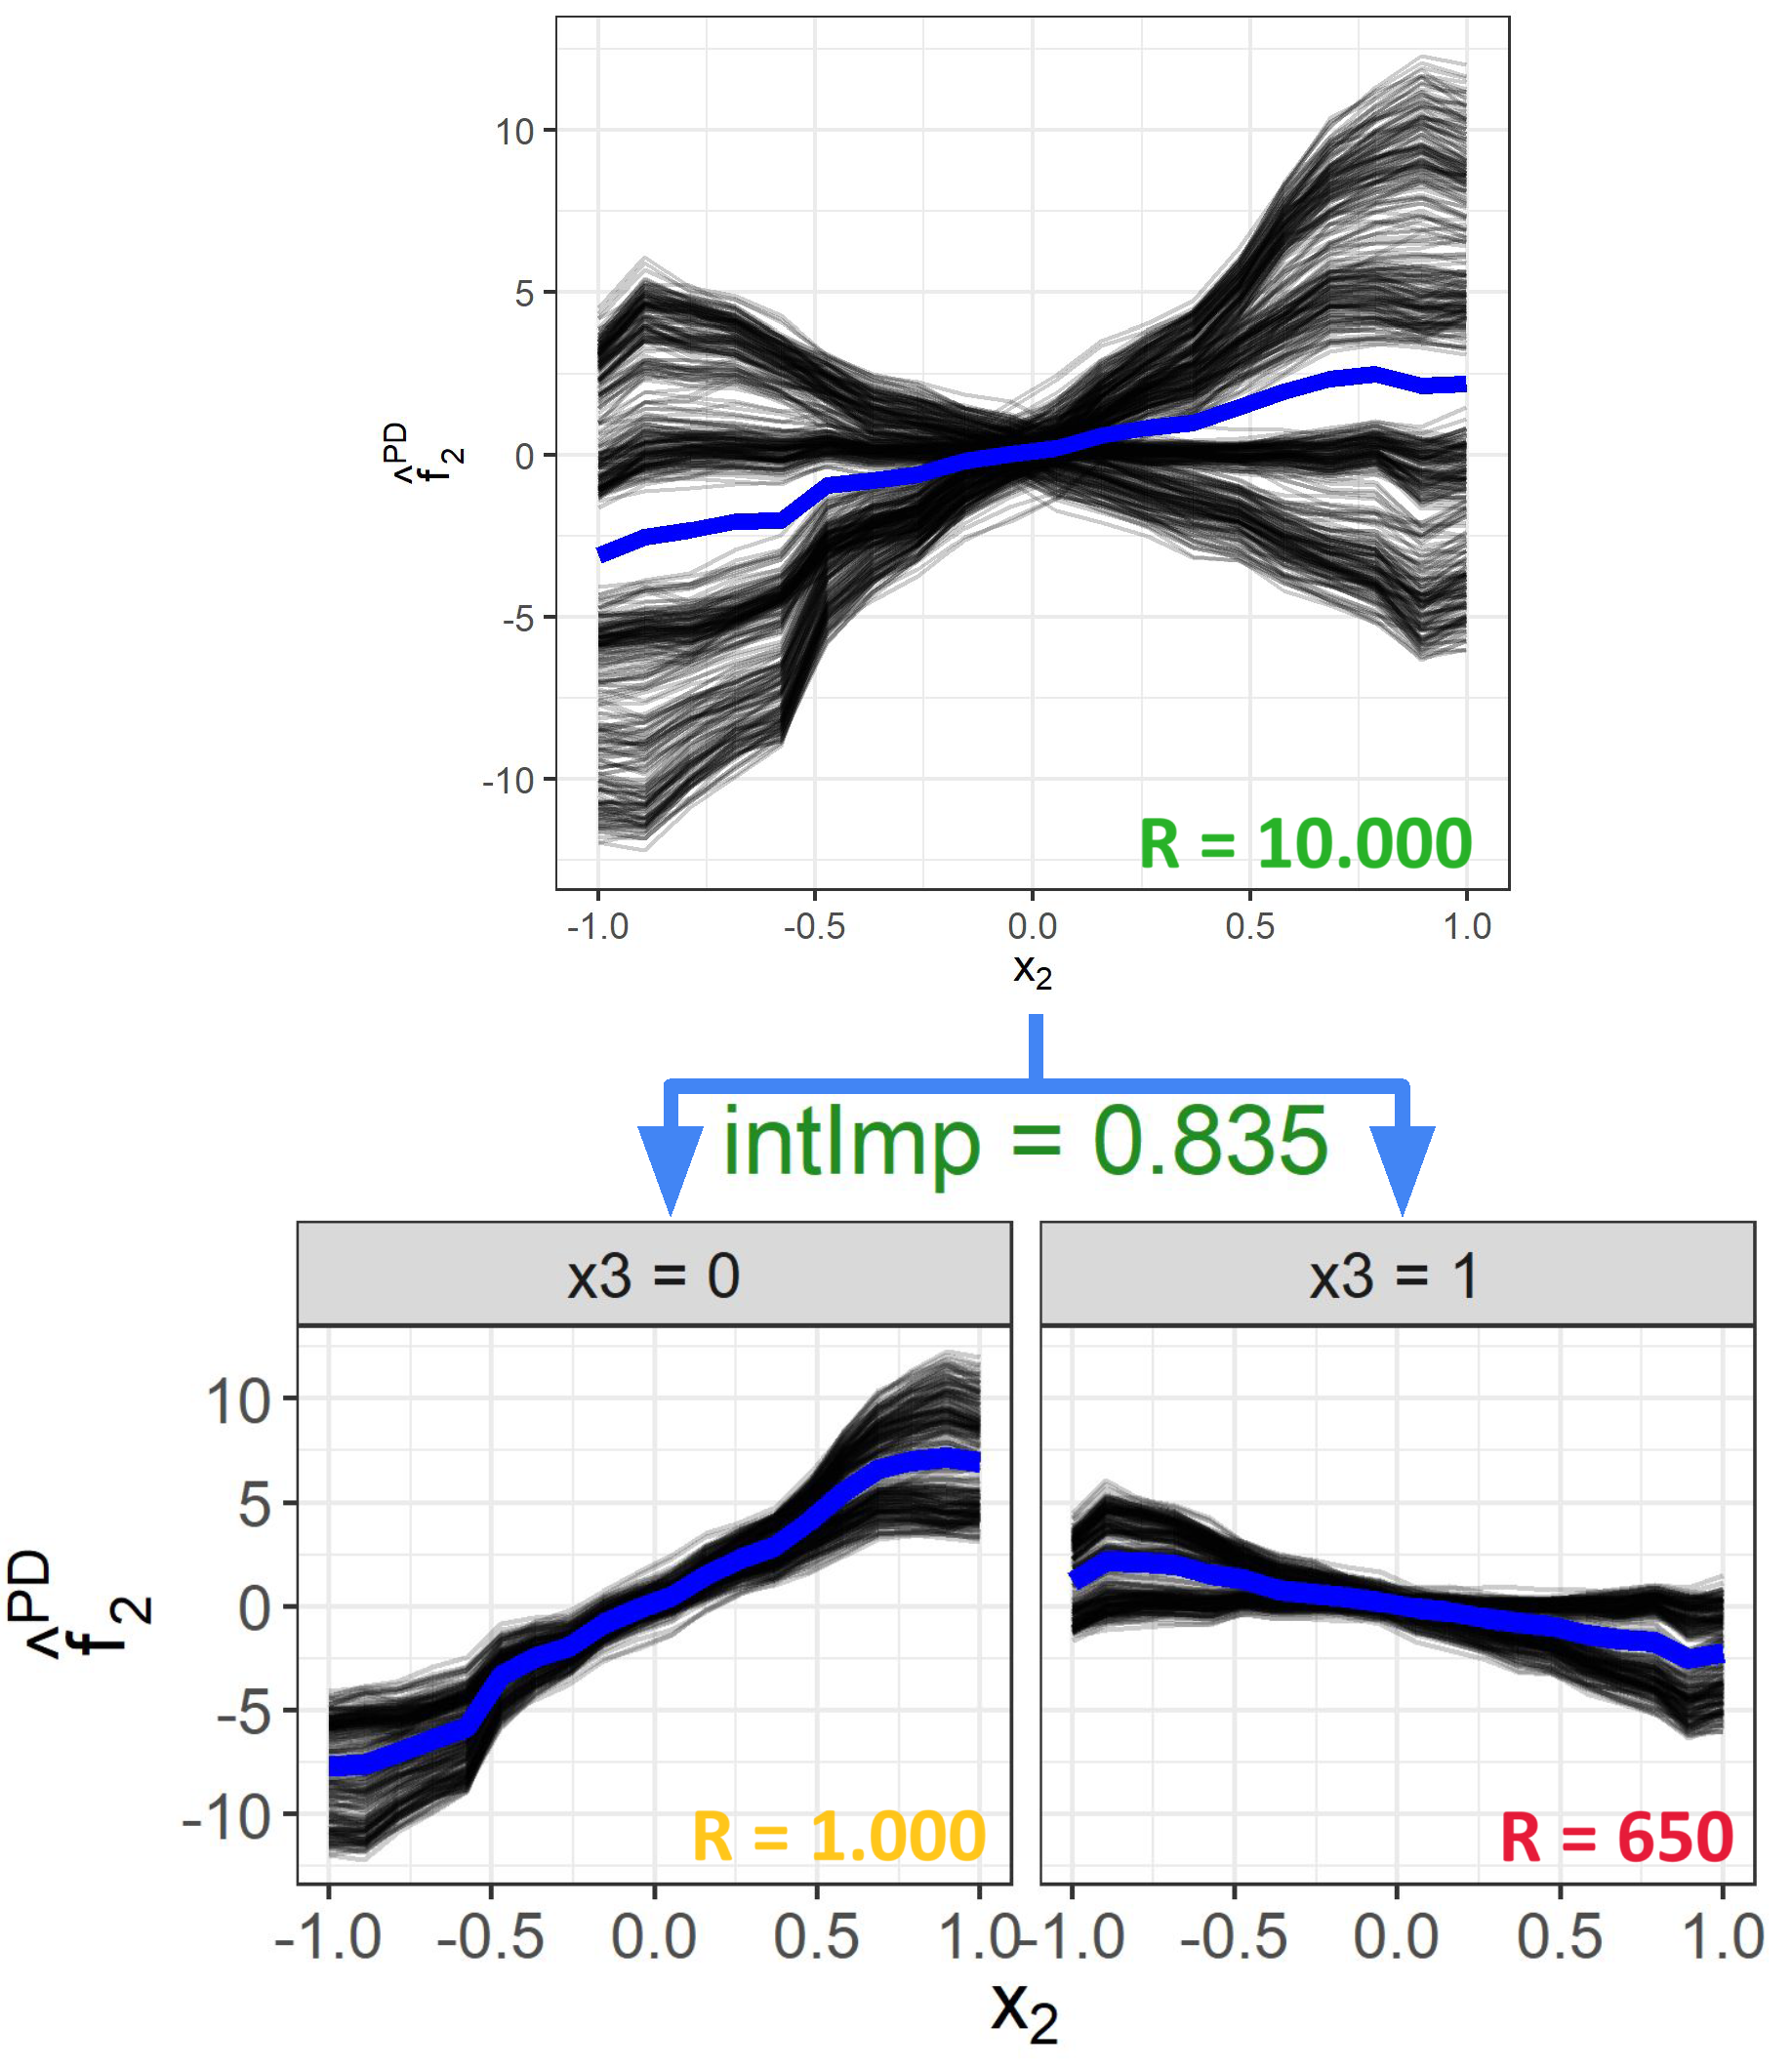
\includegraphics[width = 0.95\textwidth]{figure/sim1_fake.png}

Split reduces 83.5\% of variance.
    \end{column}
\end{columns}

\end{frame}





\begin{frame}{Interaction quantification}
    
\begin{columns}[T, totalwidth=\textwidth]%, totalwidth=\textwidth]
    \begin{column}{0.46\textwidth}

\textbf{On feature level (for $x_j$):} 
%Relative interaction importance for feature $x_j$:
%We denote this subset by $\mathcal{B}_j \subset \mathcal{B}_P$ and the relative interaction importance by
\medskip

\centerline{$\textstyle
   intImp_j = \sum\nolimits_{i \in \mathcal{B}_j} intImp(\mathcal{N}_i)$}

\medskip

%\textbf{$\bm{intImp(\mathcal{N}_P)}$: risk reduction after one split relative to the root node risk}
%where $\mathcal{B}_j$ indexes parent nodes where splits are based on $x_j$.
where $\mathcal{B}_j$ indexes parent nodes split by $x_j$.

\medskip

\textbf{Interpretation:}
Overall reduction of ICE curve variance due to splits by $X_j$ (in \%).

\medskip

\textbf{Example:} For $X_1 \Rightarrow$  {\color{orange} $\mathcal{B}_1 = \{0, 2, 3\}$}
    \begin{center}
      \resizebox{1\textwidth}{!}{
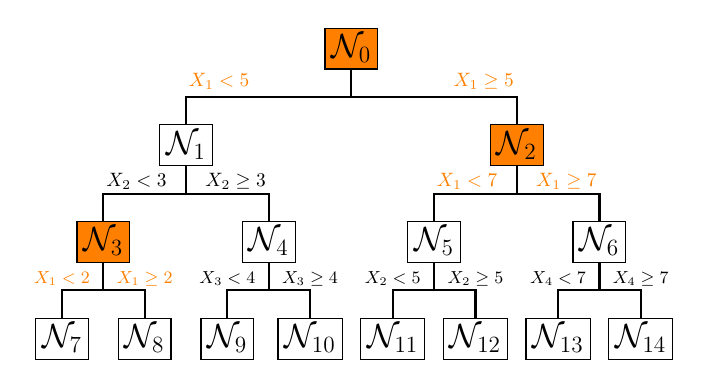
\begin{tikzpicture}[scale=0.7, transform shape]
    \tikzset{treenode/.style={draw, rectangle, font=\LARGE}}
    \tikzset{line/.style={draw, thick}}

    % Root node
    \node [treenode, fill=orange] (a0) {$\mathcal{N}_0$};

    % Level 1 nodes
    \node [treenode, below=1cm of a0, xshift=-3cm] (a1) {$\mathcal{N}_1$};
    \node [treenode, fill=orange, below=1cm of a0, xshift=3cm] (a2) {$\mathcal{N}_2$};

    % Level 2 nodes
    \node [treenode, fill=orange, below=1cm of a1, xshift=-1.5cm] (a3) {$\mathcal{N}_3$};
    \node [treenode, below=1cm of a1, xshift=1.5cm] (a4) {$\mathcal{N}_4$};
    \node [treenode, below=1cm of a2, xshift=-1.5cm] (a5) {$\mathcal{N}_5$};
    \node [treenode, below=1cm of a2, xshift=1.5cm] (a6) {$\mathcal{N}_6$};

    % Level 3 nodes
    \node [treenode, below=1cm of a3, xshift=-0.75cm] (a7) {$\mathcal{N}_7$};
    \node [treenode, below=1cm of a3, xshift=0.75cm] (a8) {$\mathcal{N}_8$};
    \node [treenode, below=1cm of a4, xshift=-0.75cm] (a9) {$\mathcal{N}_9$};
    \node [treenode, below=1cm of a4, xshift=0.75cm] (a10) {$\mathcal{N}_{10}$};
    \node [treenode, below=1cm of a5, xshift=-0.75cm] (a11) {$\mathcal{N}_{11}$};
    \node [treenode, below=1cm of a5, xshift=0.75cm] (a12) {$\mathcal{N}_{12}$};
    \node [treenode, below=1cm of a6, xshift=-0.75cm] (a13) {$\mathcal{N}_{13}$};
    \node [treenode, below=1cm of a6, xshift=0.75cm] (a14) {$\mathcal{N}_{14}$};

    % Edges and labels
    \path [line] (a0.south) -- + (0,-0.5cm) -| (a1.north) node [pos=0.4, above, color=orange] {$X_1 < 5$};
    \path [line] (a0.south) -- + (0,-0.5cm) -| (a2.north) node [pos=0.4, above, color=orange] {$X_1 \geq 5$};

    \path [line] (a1.south) -- + (0,-0.5cm) -| (a3.north) node [pos=0.3, above, yshift = -0.05cm] {$X_2 < 3$};
    \path [line] (a1.south) -- + (0,-0.5cm) -| (a4.north) node [pos=0.3, above, yshift = -0.05cm] {$X_2 \geq 3$};

    \path [line] (a2.south) -- + (0,-0.5cm) -| (a5.north) node [pos=0.3, above, color=orange, yshift = -0.05cm] {$X_1 < 7$};
    \path [line] (a2.south) -- + (0,-0.5cm) -| (a6.north) node [pos=0.3, above, color=orange, yshift = -0.05cm] {$X_1 \geq 7$};

    \path [line] (a3.south) -- + (0,-0.5cm) -| (a7.north) node [pos=0.5, above, color=orange, yshift = -0.05cm] {\small $X_1 < 2$};
    \path [line] (a3.south) -- + (0,-0.5cm) -| (a8.north) node [pos=0.5, above, color=orange, yshift = -0.05cm] {\small $X_1 \geq 2$};

    \path [line] (a4.south) -- + (0,-0.5cm) -| (a9.north) node [pos=0.5, above, yshift = -0.05cm] {\small $X_3 < 4$};
    \path [line] (a4.south) -- + (0,-0.5cm) -| (a10.north) node [pos=0.5, above, yshift = -0.05cm] {\small $X_3 \geq 4$};

    \path [line] (a5.south) -- + (0,-0.5cm) -| (a11.north) node [pos=0.5, above, yshift = -0.05cm] {\small $X_2 < 5$};
    \path [line] (a5.south) -- + (0,-0.5cm) -| (a12.north) node [pos=0.5, above, yshift = -0.05cm] {\small $X_2 \geq 5$};

    \path [line] (a6.south) -- + (0,-0.5cm) -| (a13.north) node [pos=0.5, above, yshift = -0.05cm] {\small $X_4 < 7$};
    \path [line] (a6.south) -- + (0,-0.5cm) -| (a14.north) node [pos=0.5, above, yshift = -0.05cm] {\small $X_4 \geq 7$};

\end{tikzpicture}}
    \end{center}
    \end{column}
\pause
    \begin{column}{0.52\textwidth}


    \centering
    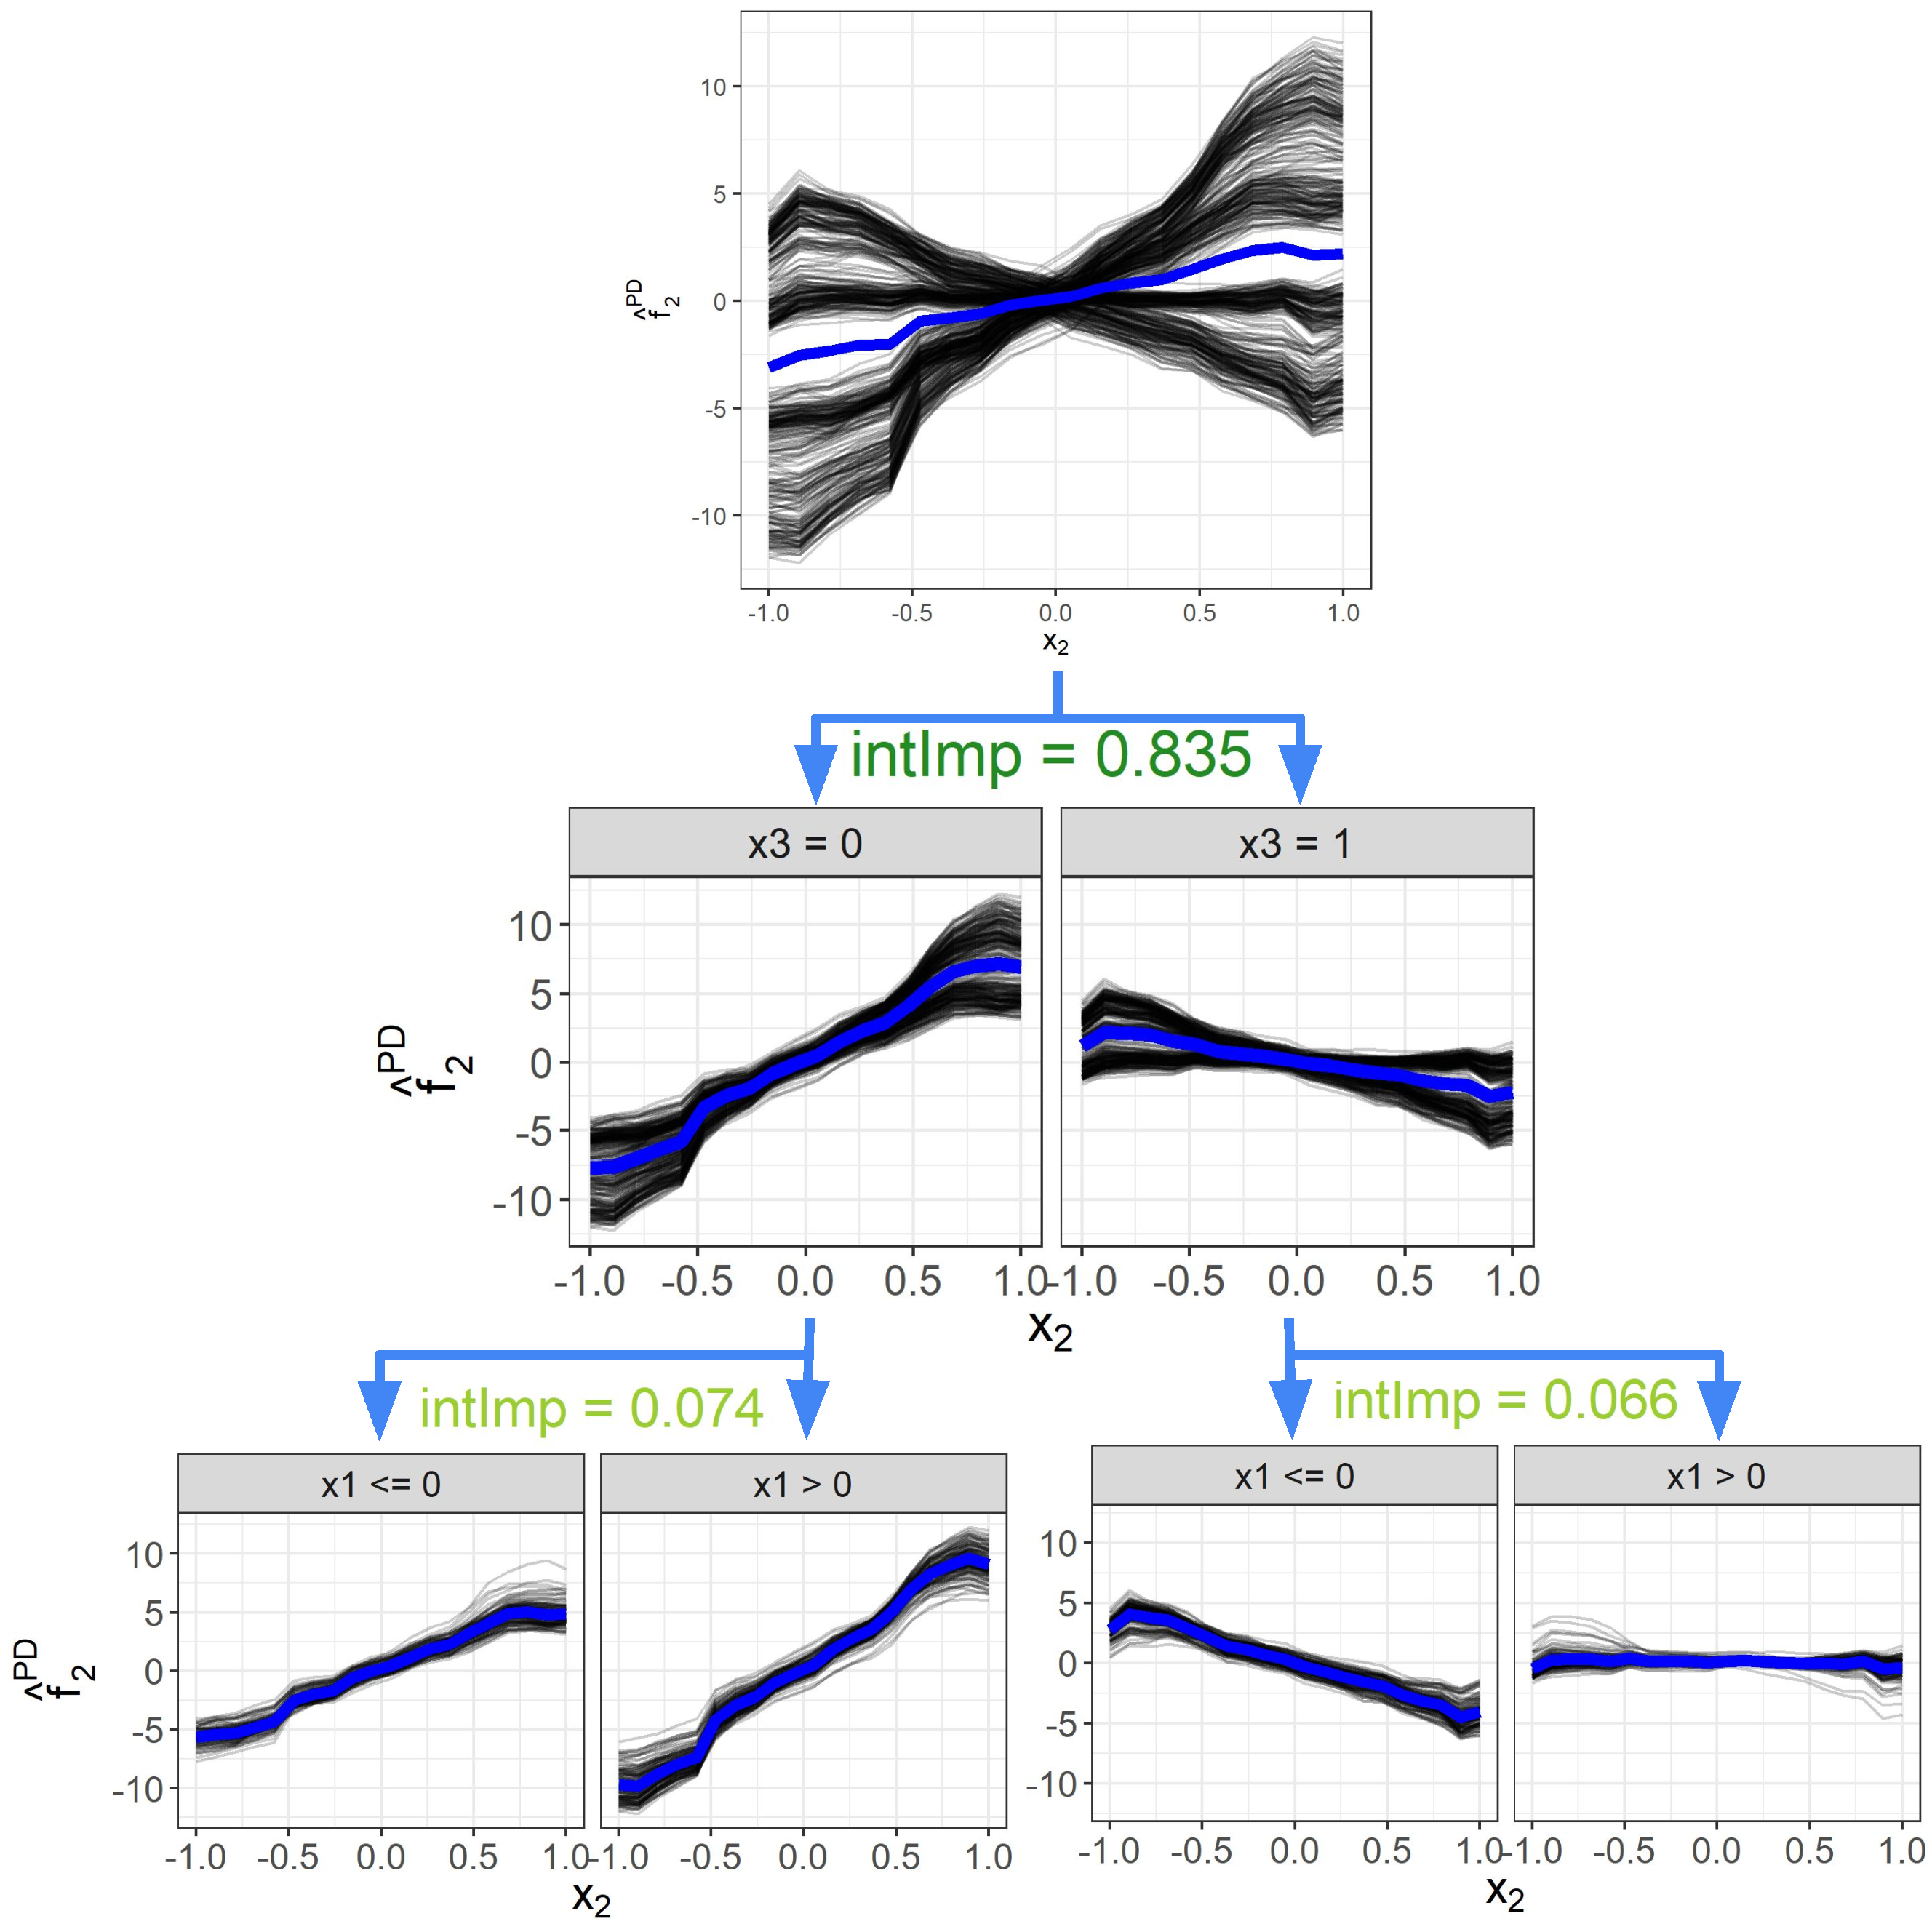
\includegraphics[width=\textwidth]{figure/sim1}
     %\begin{minipage}[t]{.5\textwidth}
    %   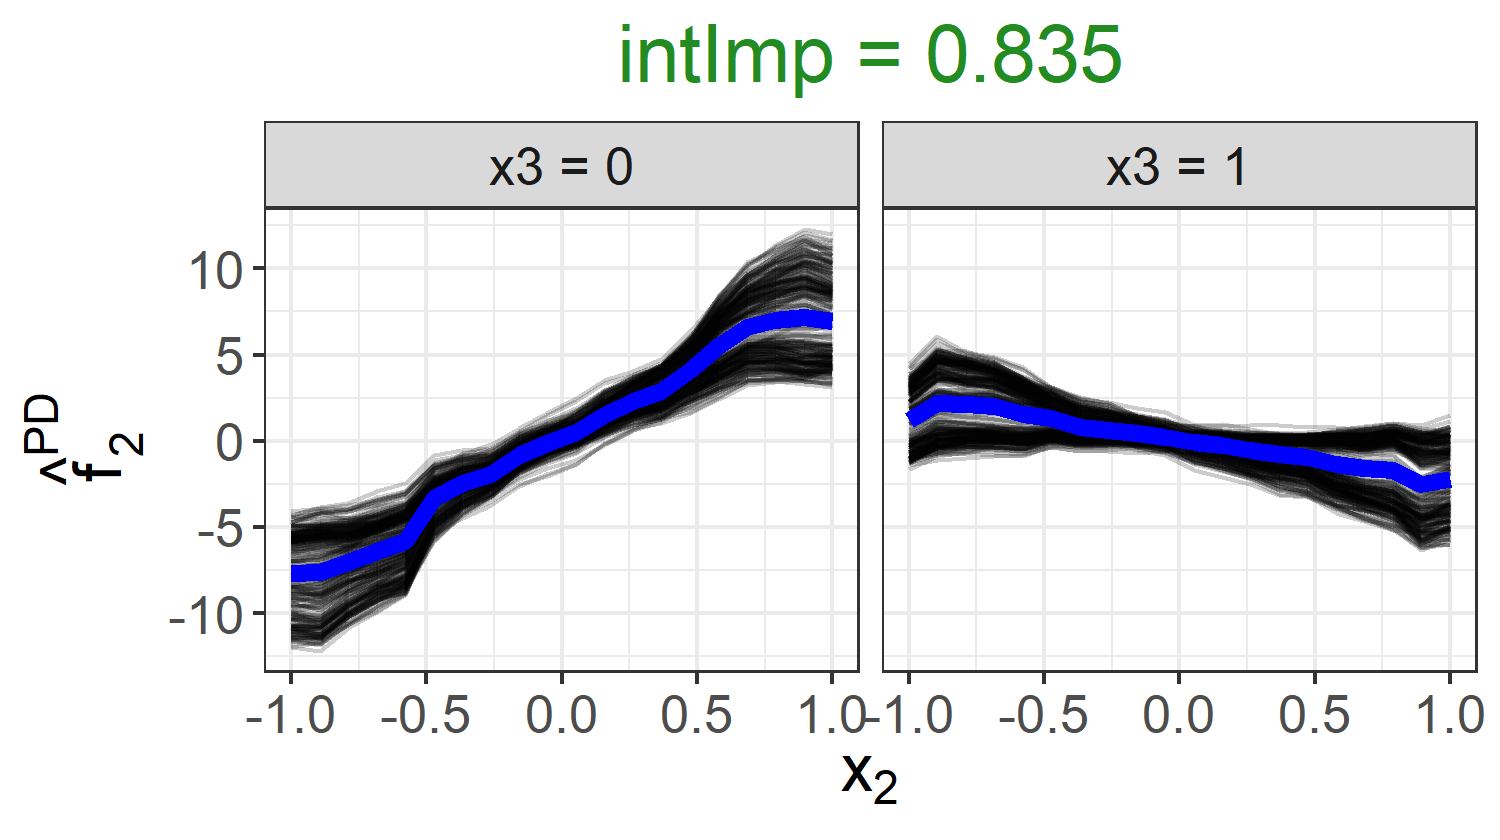
\includegraphics[width=0.37\textwidth]{figure/sim1_dt_split1.png}
    %   \scalebox{1}{
    %   \hspace{15pt} 
    %   \begin{tikzpicture}
    %   \usetikzlibrary{arrows}
    %     \usetikzlibrary{shapes}
    %      \tikzset{treenode/.style={draw}}
    %      \tikzset{line/.style={draw, thick}}
    %     \node [treenode](a0) {} ; [below=1pt,at=(4,0)]  {};
    %      \node [treenode, below=0.3cm, at=(a0.south), xshift=-1.3cm]  (a1) {};
    %      \node [treenode, below=0.3cm, at=(a0.south), xshift=-0.2cm]  (a2) {};
    %      \path [line] (a0.south) -- + (0,-0.2cm) -| (a1.north) node [midway, above] {};
    %      \path [line] (a0.south) -- +(0,-0.2cm) -|  (a2.north) node [midway, above] {};
    %   \end{tikzpicture}
    %   \hspace{25pt}
    %   \begin{tikzpicture}
    %   \usetikzlibrary{arrows}
    %     \usetikzlibrary{shapes}
    %      \tikzset{treenode/.style={draw}}
    %      \tikzset{line/.style={draw, thick}}
    %     \node [treenode] (a01) {};[below=5pt,at=(node1.south) , xshift=0cm]
    %      \node [treenode, below=0.3cm, at=(a01.south), xshift=0.1cm]  (a1) {};
    %      \node [treenode, below=0.3cm, at=(a01.south), xshift=1.1cm]  (a2) {};
    %      \path [line] (a01.south) -- + (0,-0.2cm) -| (a1.north) node [midway, above] {};
    %      \path [line] (a01.south) -- +(0,-0.2cm) -|  (a2.north) node [midway, above] {};
    %   \end{tikzpicture}
    %   }
    % 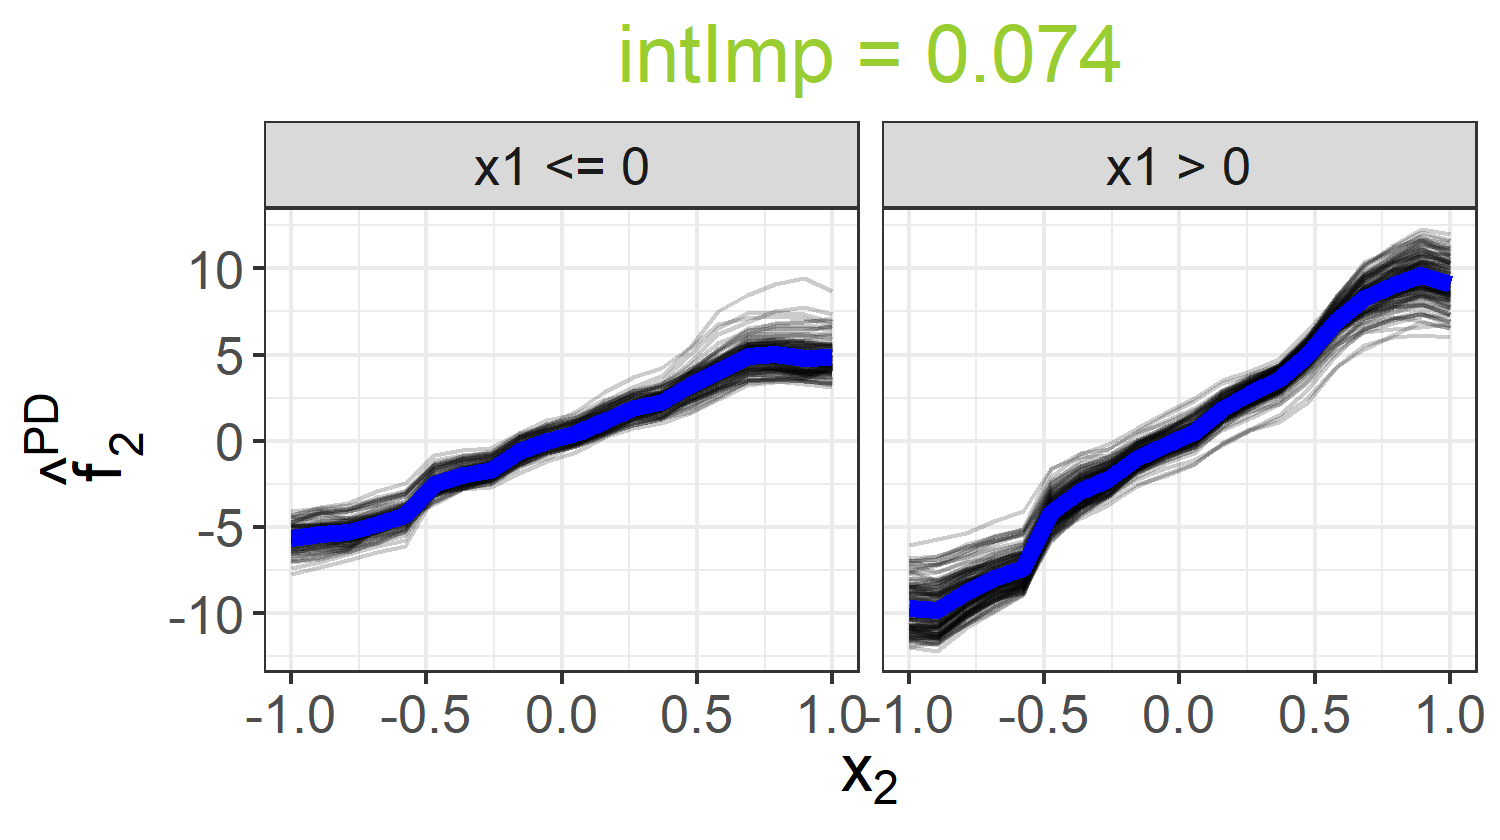
\includegraphics[width=0.37\textwidth]{figure/sim1_dt_split2_1.png}
    % 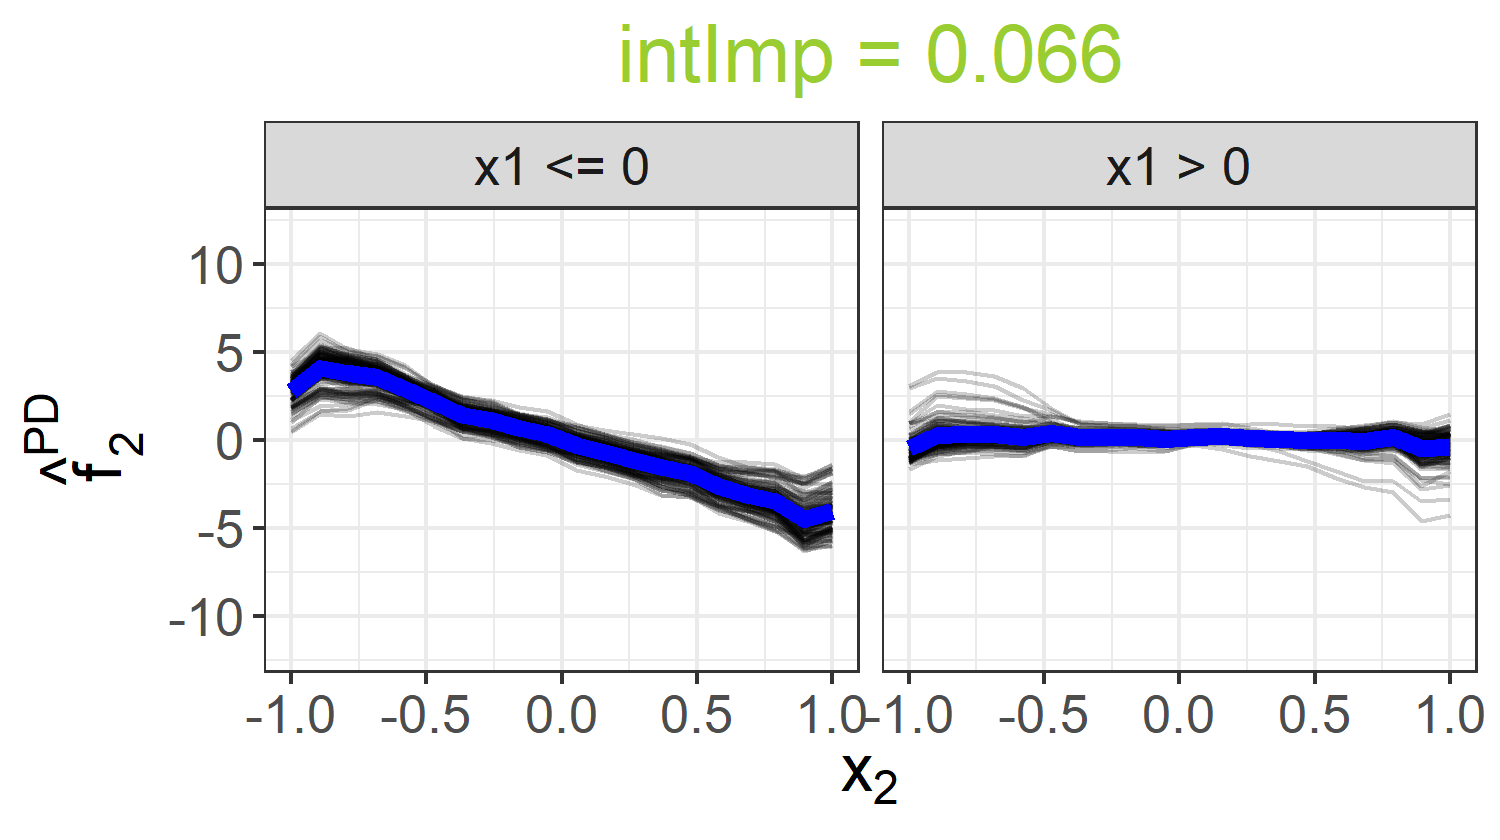
\includegraphics[width=0.37\textwidth]{figure/sim1_dt_split2_2.png}
    
 \vspace{-200px}
    \scriptsize
 \hspace{130px}
 \setlength{\tabcolsep}{1pt}
 \begin{tabular}{|c|c|}
    \hline
       $x_j$ & $intImp_j$  \\\hline
       \rowcolor{ForestGreen!70}
        $\xv_3$     & 0.835 \\
        \rowcolor{YellowGreen!50}
        $\xv_1$     &  0.14\\\hline
    \end{tabular}\\
 \hspace{138px}= 0.975
      %\footnotesize\\
    %\vspace{150px}

    \end{column}
\end{columns}

\end{frame}





\begin{frame}{Outperforming SOTA}

\textbf{Simulation setting}
\begin{itemize}
    \item Draw 1000 i.i.d. samples from $X_1, \ldots , X_4 \sim \mathcal{U}(-1,1)$
    \item True underlying function: $f(\xv) = \sum\nolimits_{j=1}^4 \xv_j + \xv_1 \xv_2 + \xv_2 \xv_3 + \xv_1 \xv_3 + \xv_1 \xv_2 \xv_3 + \epsilon$ % , \epsilon \sim \mathbbm{N}(0, 0.01 \sigma(\mu(\xv))^2)
    \item Fit a correctly specified linear model (interactions with $\xv_4$ are excluded)
    \item 30 repetitions, measure interaction strength between $\xv_2$ and all other 3 features
\end{itemize}

\textbf{Which methods are sensitive to changes in main effect sizes or feature correlations?}


    \begin{table}[thb]
\vspace{.1in}
    \label{tab:simSummary}
    \begin{center}
    \begin{tabular}{|p{5.4cm}|p{1.6cm}|p{1.8cm}|p{1.6cm}|p{1.6cm}|}
    \hline
       Pitfall & REPID & H-Statistic & Greenwell & SHAP  \\\hline
       sensitive to changes of main effect & No & Yes & Yes & No\\\hline
       sensitive to changes of correlation between $\xv_j$ and other features & No & Yes & No & Yes\\
  \hline
    \end{tabular}
    \end{center}
\end{table}
\vspace*{0.2cm}




\end{frame}

\begin{frame}{Outperforming SOTA}
\centerline{
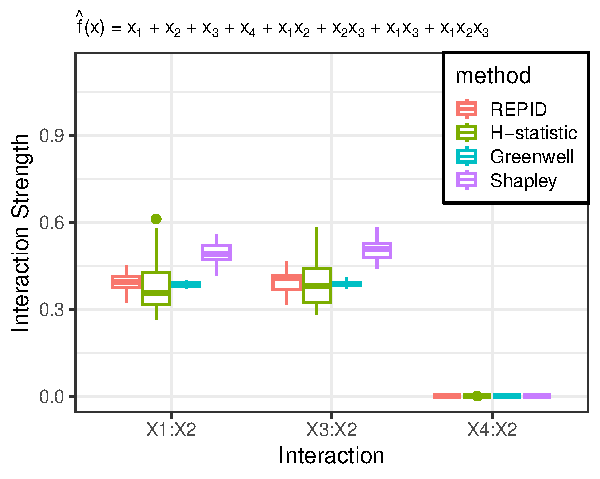
\includegraphics[width=0.4\textwidth, page = 1]{figure/sim_sensi_linear.pdf}
\includegraphics[width=0.4\textwidth, page = 2]{figure/sim_sensi_linear.pdf}
}

   \begin{itemize}
       \item \textbf{Left (initial setting)}: Interaction strength of $\xv_1$:$\xv_2$ and $\xv_3$:$\xv_2$ similar; $\xv_4$:$\xv_2$ no interaction
       \item \textbf{Right}: Set main effect $\beta_1$ = 0.1
       
   \begin{itemize}
       \item \textbf{Expectation}: Interaction strengths should not change
       \item \textbf{Fail}: H-statistic ($\xv_1$:$\xv_2$ > $\xv_3$:$\xv_2$) and Greenwell ($\xv_1$:$\xv_2$ < $\xv_3$:$\xv_2$) 
   \end{itemize}
   \end{itemize}
\end{frame}

\begin{frame}{Outperforming SOTA}
\centerline{
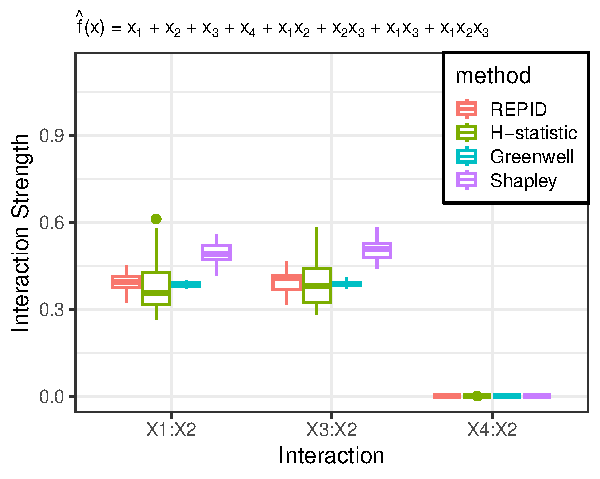
\includegraphics[width=0.4\textwidth, page = 1]{figure/sim_sensi_linear.pdf}
\includegraphics[width=0.4\textwidth, page = 3]{figure/sim_sensi_linear.pdf}
}
  \begin{itemize}
        \item \textbf{Left (initial setting)}: Interaction strength of $\xv_1$:$\xv_2$ and $\xv_3$:$\xv_2$ similar; $\xv_4$:$\xv_2$ no interaction
       \item \textbf{Right}: Increase correlation $\rho(\xv_1, \xv_2) = 0.9$
          \begin{itemize}
       \item \textbf{Expectation}: Interaction strengths should not change
       \item \textbf{Fail}: H-statistic ($\xv_1$:$\xv_2$ < $\xv_3$:$\xv_2$) and Shapley ($\xv_1$:$\xv_2$ > $\xv_3$:$\xv_2$)
   \end{itemize}
       \item[$\rightarrow$] \textbf{REPID is the only method which always leads to correct rankings for these settings}  
   \end{itemize}
   
\end{frame}





\begin{frame}{Limitations of REPID}

\begin{columns}[T, totalwidth = \textwidth]
    \begin{column}{0.48\textwidth}

%\pause
% \textbf{Limitations}:
      \begin{itemize}
  \item[1)] Restricted to one feature of interest \\
  $\Rightarrow$ Different regions for different features \\
  %$\Rightarrow$ No unique decomposition of $\hat{f}(x)$\\%iction function possible\\
  %\item Restricted to ICE curves and PDs $\rightarrow$ not flexible w.r.t. feature effect method
  %\pause
  \item<2->[2)] Restricted to PD (global) and ICE (local) as feature effect methods\\
  $\Rightarrow$ Inherits extrapolation problem\\
  %\phantom{$\Rightarrow$} 
  (unlikely combinations of feature values)
      %\item Feature effect methods based on integrating over marginal distributions such as ICE and PD might extrapolate in unseen or sparse regions (e.g., small $\xv_1$ and high $\xv_3$ values)
      %\item Global/regional effects are not representative w.r.t. the data distribution  
   \item<2->[$\leadsto$] Follow-up GADGET %``Generalized Additive Decomposition of Global feature EffecTs based on interactions'' 
[under review]
  \end{itemize}


        % \begin{itemize}
        %     \item $f(X) = 3X_1\mathbbm{1}_{X_3>0} - 3X_1\mathbbm{1}_{X_3\leq 0} + X_3 + \epsilon$
        %     \item Features uniformly distributed
        %     \item Left: features independent
        %     \item Right: $X_1$ and $X_3$ highly correlated
        %     \item First split: $\xv_3 \leq 0$ (blue) and $\xv_3 > 0$ (orange)
        % \end{itemize}
    \end{column}

    \only<1>{   \begin{column}{0.52\textwidth}
    \centering
    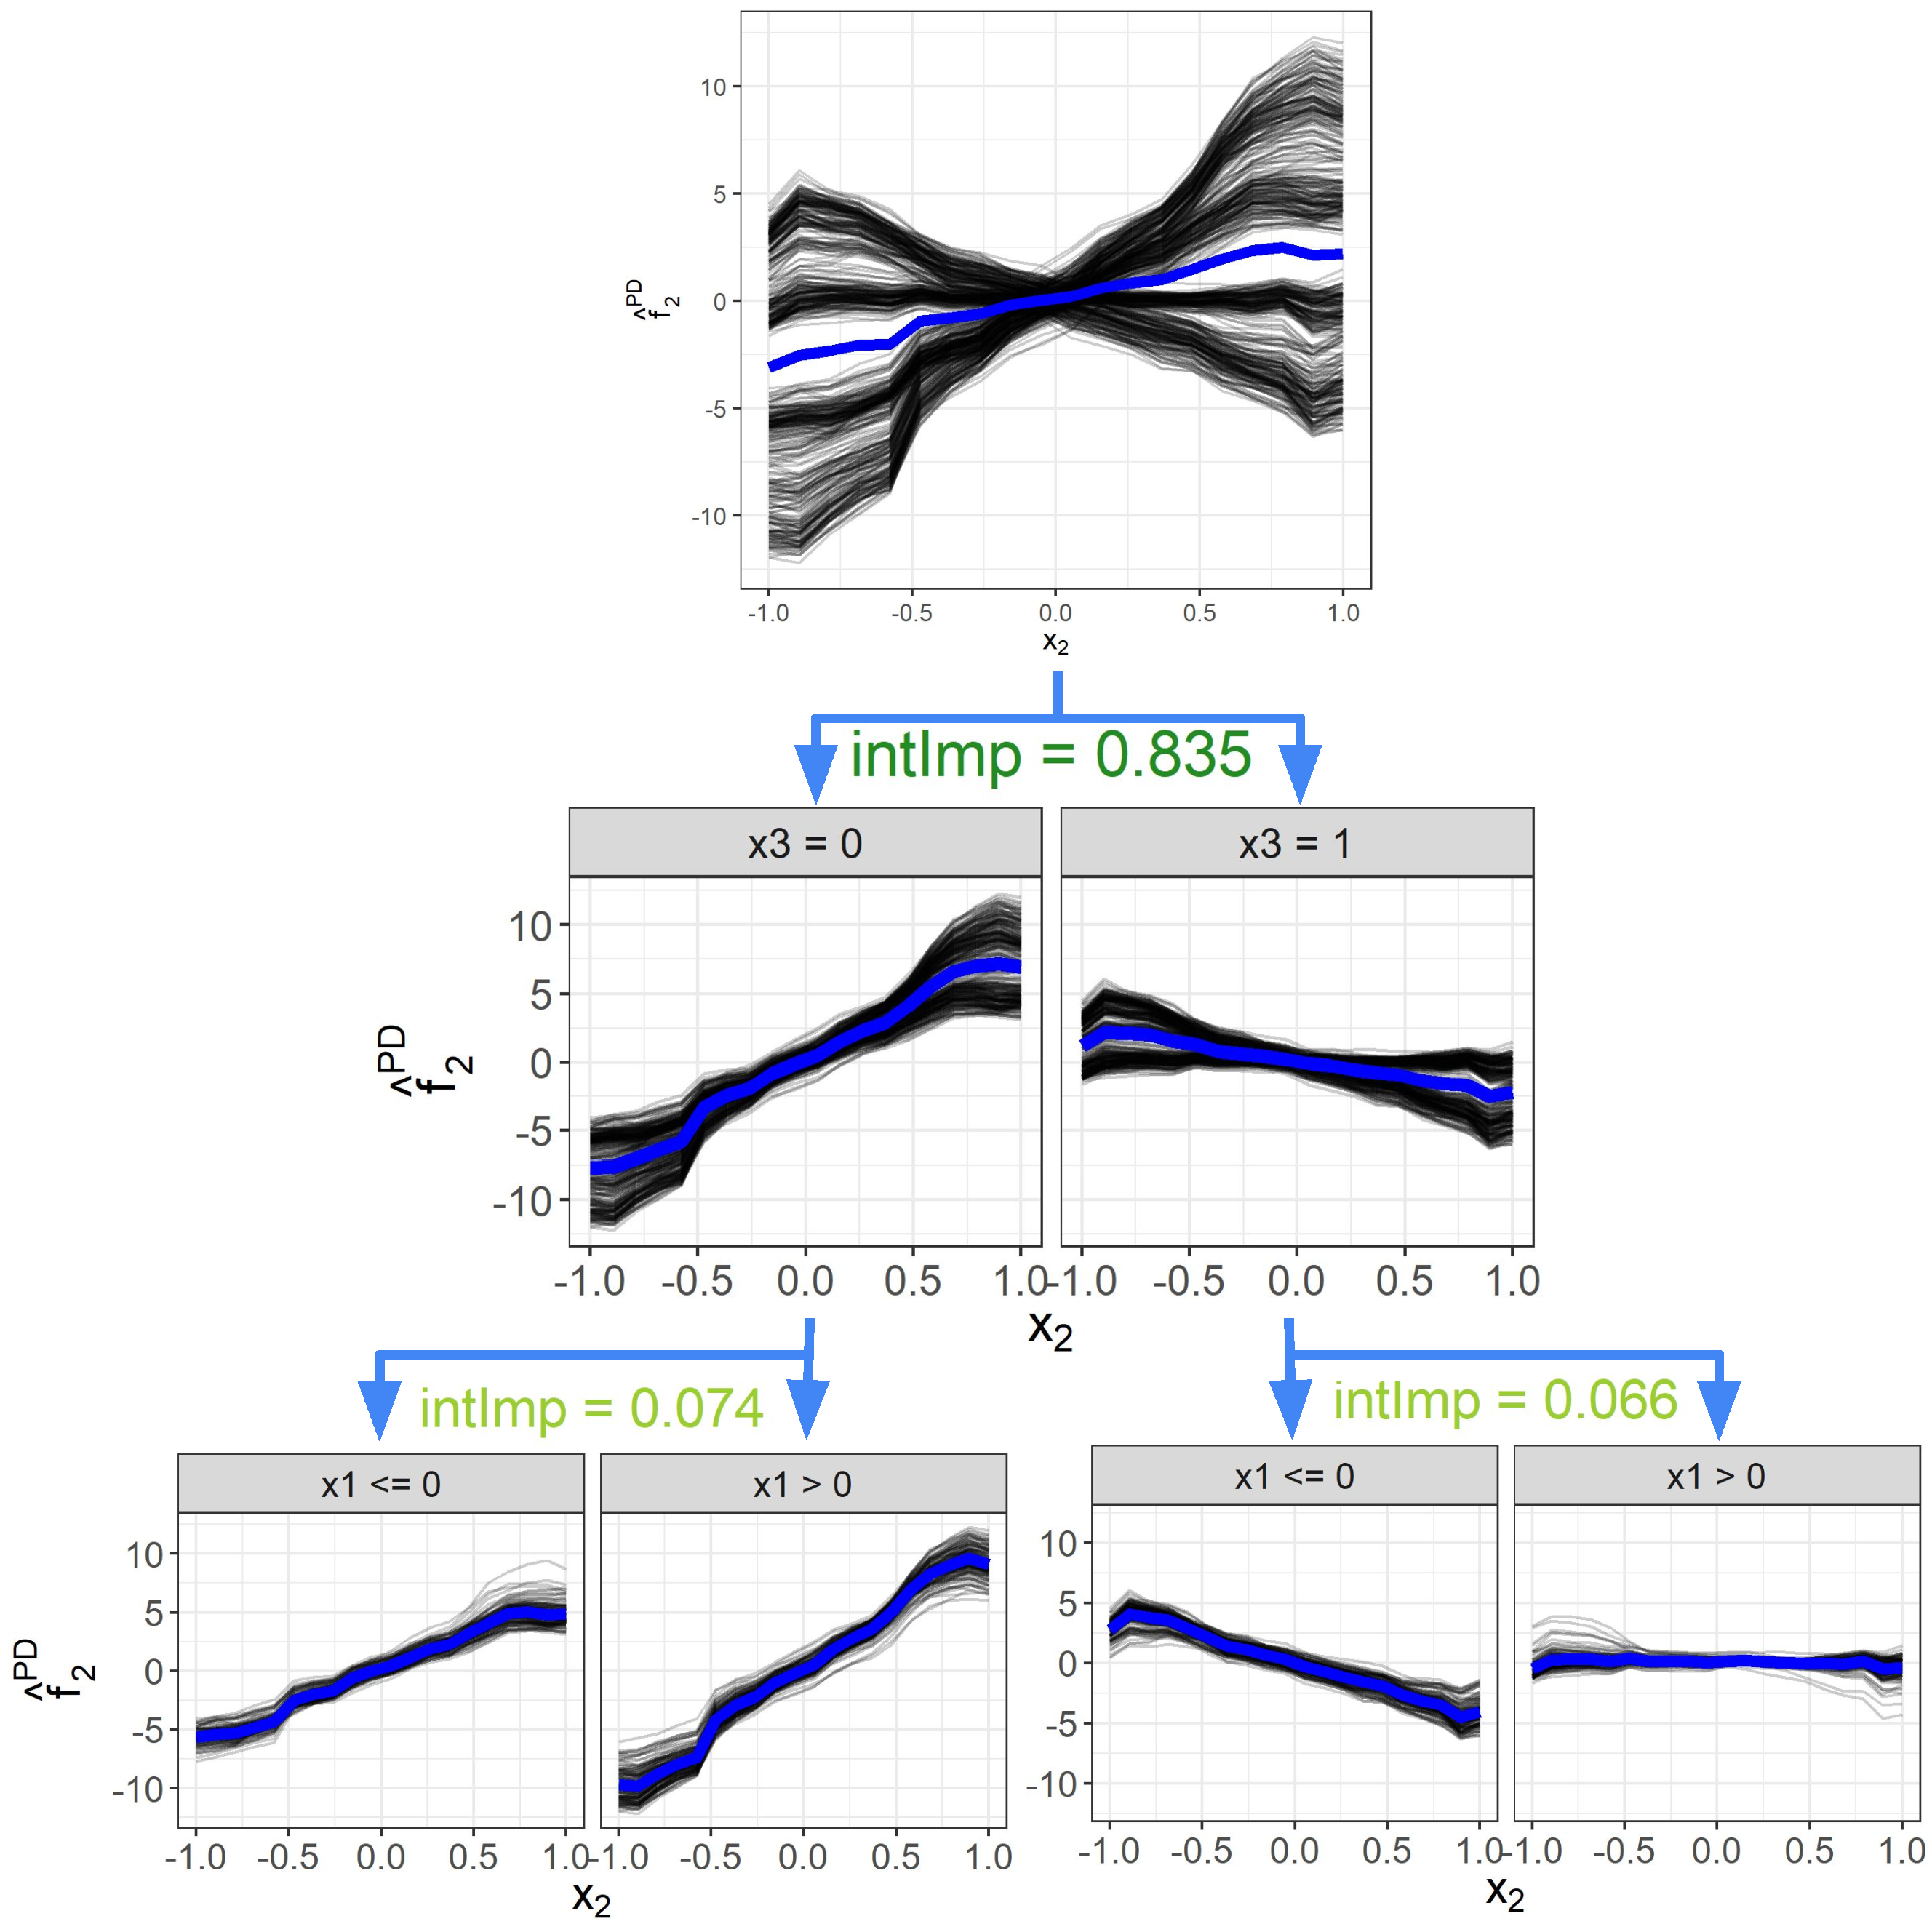
\includegraphics[width=0.95\textwidth]{figure/sim1}
    \vspace{-8pt}
        \begin{columns}[T, totalwidth = \linewidth]
     \footnotesize
            \begin{column}{0.125\linewidth}
            \centering
             $\hat{f}_2^{PD}(X_2)$ %, X_1 > 0 \land X_3 = 0\)\\
         \end{column}
         \begin{column}{0.175\linewidth}
         \centering
             $\approx 8X_2$ %, X_1 > 0 \land X_3 = 0\)\\
         \end{column}
        \begin{column}{0.225\linewidth}
\centering
            $\approx 16X_2$ %, X_1 \leq 0 \land X_3 = 0\)
         \end{column}
        \begin{column}{0.225\linewidth}
        \centering
            $ \approx -8X_2$ %, X_1 \leq 0 \land X_3 \neq 0\)
         \end{column}        
         \begin{column}{0.225\linewidth}
         \centering
             $\approx 0$%, X_1 > 0 \land X_3 \neq 0\)\\
         \end{column}
        \begin{column}{0.025\linewidth}

         \end{column}
     \end{columns}
    \end{column}
}
    \only<2->{\begin{column}{0.52\textwidth}
        %\begin{figure}
      %   \hspace{0.025\linewidth} uncorrelated \hspace{0.225\linewidth} correlated \hspace{0.2\linewidth}
      % \includegraphics[width = \textwidth]{figure/example_repid_extrapol.pdf}
      %      $f(X) = \highlight{3X_1\mathbbm{1}_{X_3>0}} \highlightICE{- 3X_1\mathbbm{1}_{X_3\leq 0}} + X_3 + \epsilon$
      %      \begin{itemize}
      %          \item Left: $X_1, X_2, X_3 \sim \mathbbm{U}(-1,1)$ iid
      %          \item Right: $X_1 = X_3 + \epsilon_1, \epsilon_1 \sim \mathbbm{N}(0, 0.0625)$
      %          \item Model: Tuned feedforward NN
      %          \item Split: $X_3 \leq 0$ (blue), $X_3 > 0$ (orange)
      %      \end{itemize}
      \centering
 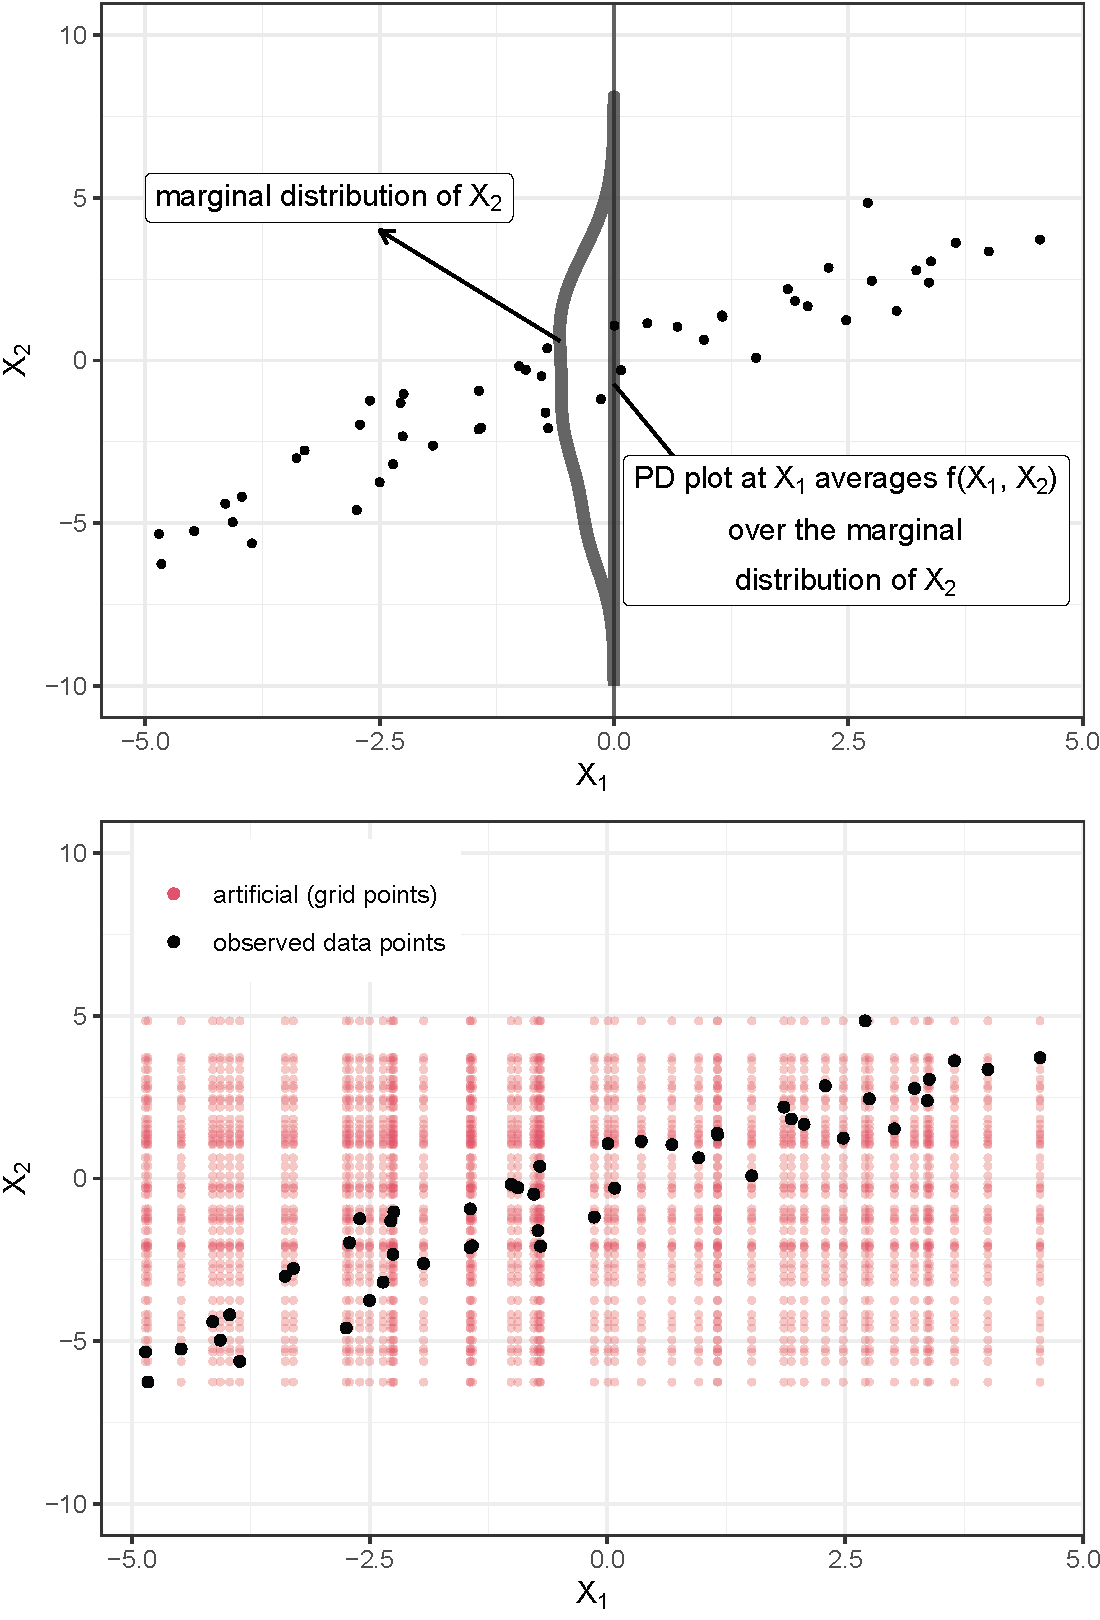
\includegraphics[width = 0.675
 \textwidth]{figure/ale_pdplot.png}
     % \caption{
      %$X_1, X_2, X_3 \sim \mathbbm{U}(-1,1)$ and 
      %$Y = 3X_1\mathbbm{1}_{X_3>0} - 3X_1\mathbbm{1}_{X_3\leq 0} + X_3 + \epsilon$% with $\epsilon \sim \mathbb{N}(0,0.09)$. 
      %left: features independent, right: $X_1$ and $X_3$ highly correlated.
      %$X_1 = X_3 + \delta$ and $\delta \sim \mathbb{N}(0, 0.0625)$. 
      %First split: $\xv_3 \leq 0$ (blue) and $\xv_3 > 0$ (orange).}
  %\end{figure}
    \end{column}}

\end{columns}
\bigskip
\end{frame}





\begin{frame}{GADGET \citebutton{Herbinger et al. (2024)}{https://www.jmlr.org/papers/v25/23-0699.html}}
\begin{itemize}
    %\item Generalized Additive Decomposition of Global feature EffecTs based on interactions
    \item[1)] Jointly minimize interactions of \textbf{multiple features} to obtain unique regions\\
    $\Rightarrow$ Additive decomposition of prediction function (if no interactions in terminal regions)
\end{itemize}

\begin{columns}[T, totalwidth = \textwidth]
    \begin{column}{0.88\textwidth}
       \begin{figure}[tbh]
    \centering
     \begin{minipage}[t]{\textwidth}
     \centering
      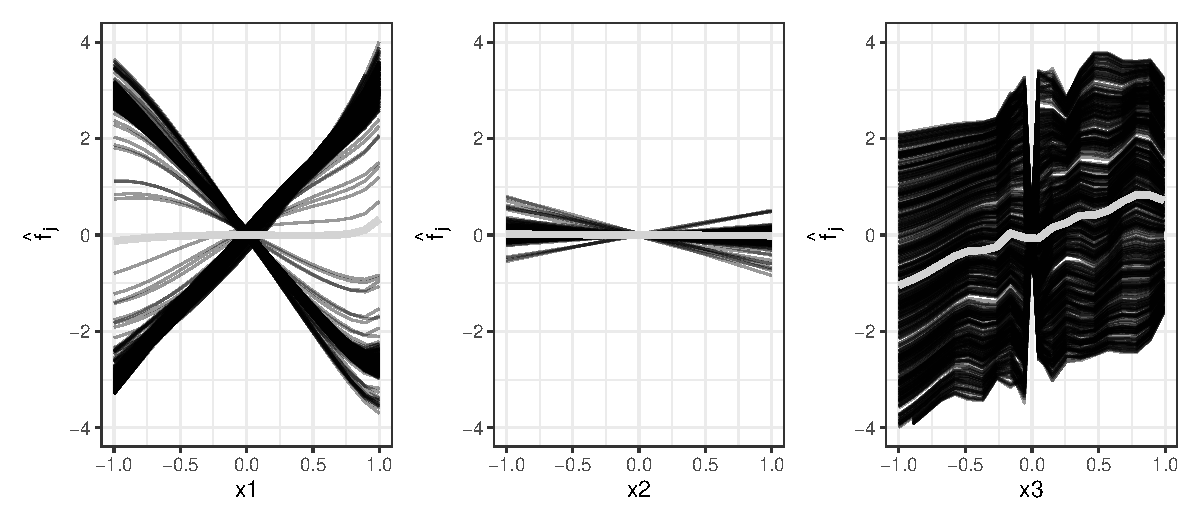
\includegraphics[width=0.49\linewidth]{figure/full_tree_root.pdf}
      \scalebox{1}{
      \hspace{15pt} 
      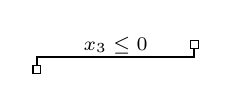
\begin{tikzpicture}
      \usetikzlibrary{arrows}
        \usetikzlibrary{shapes}
         \tikzset{treenode/.style={draw, minimum size=0.05cm, inner sep=0.05cm}}
         \tikzset{line/.style={draw, thick}}
        \node [treenode](a0) {} ; [below=1pt,at=(4,0)]  {};
         \node [treenode, below=0.2cm, at=(a0.south), xshift=-2.0cm]  (a1) {};
         %\node [treenode, below=0.3cm, at=(a0.south), xshift=-0.4cm]  (a2) {};
         \path [line] (a0.south) -- + (0,-0.1cm) -| (a1.north) node [midway, above] {};
         \node[at=(a0.south), xshift=-1cm, yshift=0.05cm]{\scriptsize $x_3 \leq 0$};
         %\path [line] (a0.south) -- +(0,-0.2cm) -|  (a2.north) node [midway, above] {};
      \end{tikzpicture}
      \hspace{35pt}
      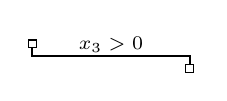
\begin{tikzpicture}
      \usetikzlibrary{arrows}
        \usetikzlibrary{shapes}
         \tikzset{treenode/.style={draw,  minimum size=0.05cm, inner sep=0.05cm}}
         \tikzset{line/.style={draw, thick}}
         %at=(node1.south)
        \node [treenode] (a01) {};[below=5pt, at=(4,0)]
         %\node [treenode, below=0.3cm, at=(a01.south), xshift=0.4cm]  (a1) {};
         \node [treenode, below=0.2cm, at=(a01.south), xshift=2cm]  (a2) {};
         %\path [line] (a01.south) -- + (0,-0.2cm) -| (a1.north) node [midway, above] {};
         \path [line] (a01.south) -- +(0,-0.1cm) -|  (a2.north) node [midway, above] {};
         \node[at=(a01.south), xshift=1cm, yshift=0.05cm]{\scriptsize $x_3 > 0$};
      \end{tikzpicture}
      }
    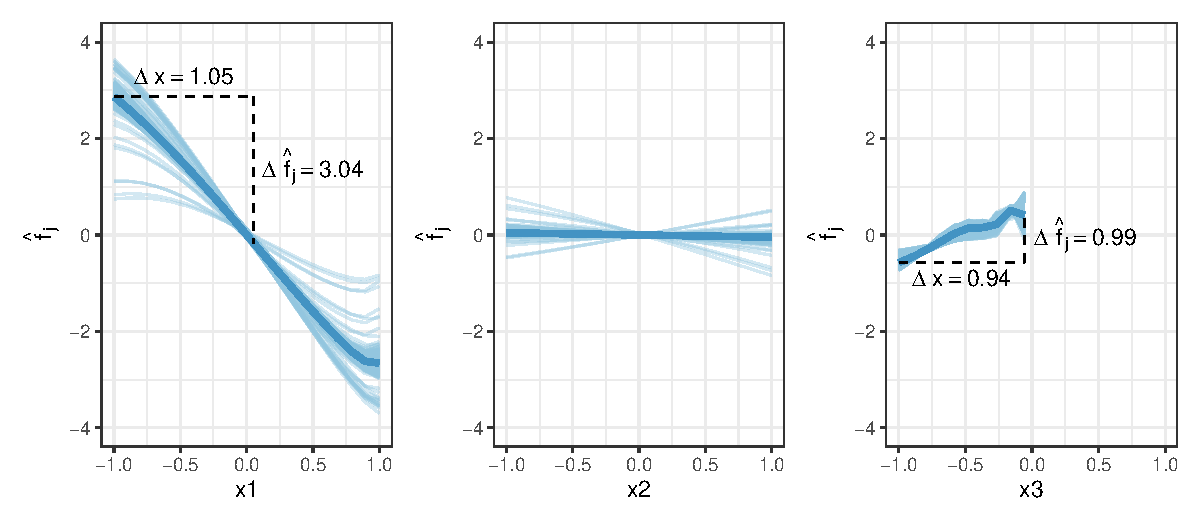
\includegraphics[width=0.495\linewidth]{figure/full_tree_left.pdf}
    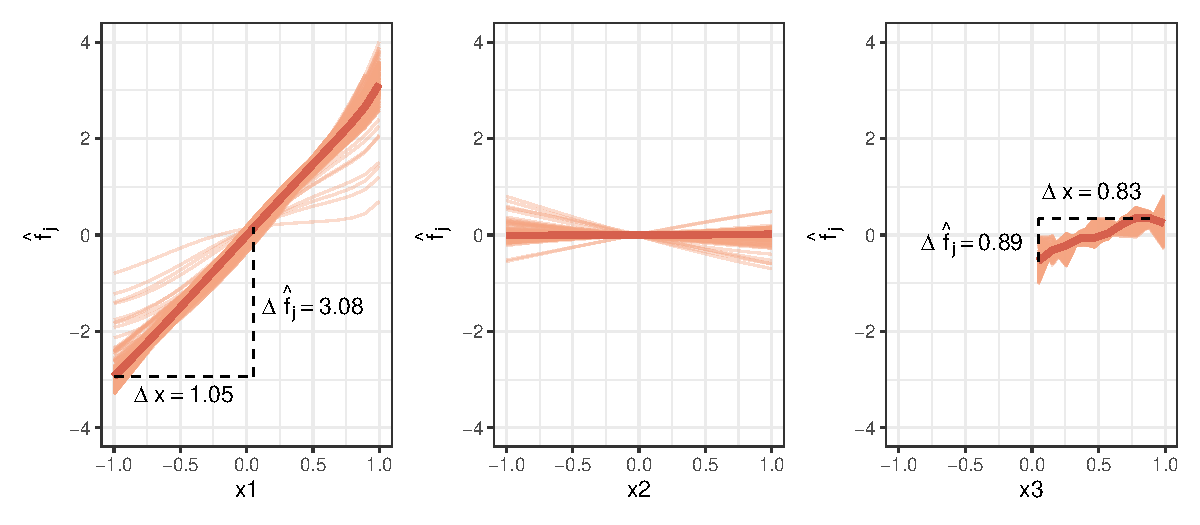
\includegraphics[width=0.495\linewidth]{figure/full_tree_right.pdf}
    %\vspace{.2in}
    %\caption{Visualization of applying GADGET with $S = Z = \{\xv_1,\xv_2,\xv_3\}$ to mean-centered ICE curves of the uncorrelated simulation example of Section \ref{sec:repid} with $Y = 3X_1\mathbbm{1}_{X_3>0} - 3X_1\mathbbm{1}_{X_3\leq 0}  + X_3 + \epsilon$ with $\epsilon \sim \mathbb{N}(0,0.09)$. The upper plots show the ICE curves and respective PD curves on the entire feature space, while the lower plots represent the respective mean-centered ICE and PD curves after partitioning the feature space w.r.t. $\xv_3 = -0.003$.
    %}
    %%\label{fig:pdp_dt}
     \end{minipage} 
\end{figure} 
    \end{column}
    \begin{column}{0.1\textwidth}
    \medskip

    \end{column}
\end{columns}

\usetikzlibrary{overlay-beamer-styles,positioning}
\begin{tikzpicture}[remember picture,overlay]
\begin{pgfonlayer}{myback}
\node [exampleblock]
at ([xshift=-3cm,yshift=-3.2cm]current page.north east) { % Adjust the shift to position the block
\scriptsize
$X_1, X_2, X_3 \sim \mathbbm{U}(-1,1)$, Model: FNN
\nodepart{two}
\scriptsize
$f(X) = 3X_1\mathbbm{1}_{X_3>0} - 3X_1\mathbbm{1}_{X_3\leq 0} + X_3 + \epsilon$
\nodepart{three}
\scriptsize
$x_3 \leq 0: \fh(\xv) \approx - 2.90 \cdot\xv_1 + 1.05\cdot \xv_3$
\nodepart{four}
\scriptsize
$x_3 > 0: \fh(\xv) \approx + 2.93 \cdot\xv_1 + 1.07\cdot \xv_3$
%\fh_{\mathcal{A}_l}(\xv) \approx g_0 - 2.9 \cdot\xv_1 + 1.05\cdot \xv_3$
};
\end{pgfonlayer}
\end{tikzpicture}
\end{frame} 



\begin{frame}{GADGET}
\begin{itemize}
    \item[2)] Support \textbf{other feature effect methods}, requirement:
    \begin{itemize}
        \item Local effect function $h$ can be aggregated to a global effect similar to ICE $\rightarrow$ PD
        \item \textbf{Axiom 1 [Local Decomposability of $h$]}:
        $$h(\tilde x_j, \xv_{-j}) = g_j(\tilde x_j) +  \sum\limits_{\substack{W \subseteq -j}} g_{W \cup j}(\tilde x_j,\xv_W)$$
        $\leadsto$ Local effect function $h$ only depends on main and higher-order effects of feature $j$ \\
        %$\leadsto$ Minimizing variance of local effect function quantifies interactions\\
        \pause
        $\leadsto$ \textbf{REPID:} Use \textbf{mean-centered ICE curve} as local effect function $h$ to meet Axiom 1 \\
        \phantom{$\leadsto$ }(uncentered ICE depends also on other effects causing vertical shift)

    \end{itemize}
    \end{itemize}    

%\footnote[frame]{\textbf{Work in progress.}}  

 \begin{columns}[T, totalwidth=\textwidth]
        \begin{column}{0.38\textwidth}
                \begin{itemize}
            \item[$\Rightarrow$] Axiom 1 is satisfied by %well-known feature effect methods:

            \begin{itemize}
            \item PD: mean-centered ICE
            \item ALE: local derivatives
            \item Shapley Dependence Plot: Shapley values
        \end{itemize}
        \end{itemize}
        \end{column}
                \begin{column}{0.61\textwidth}
    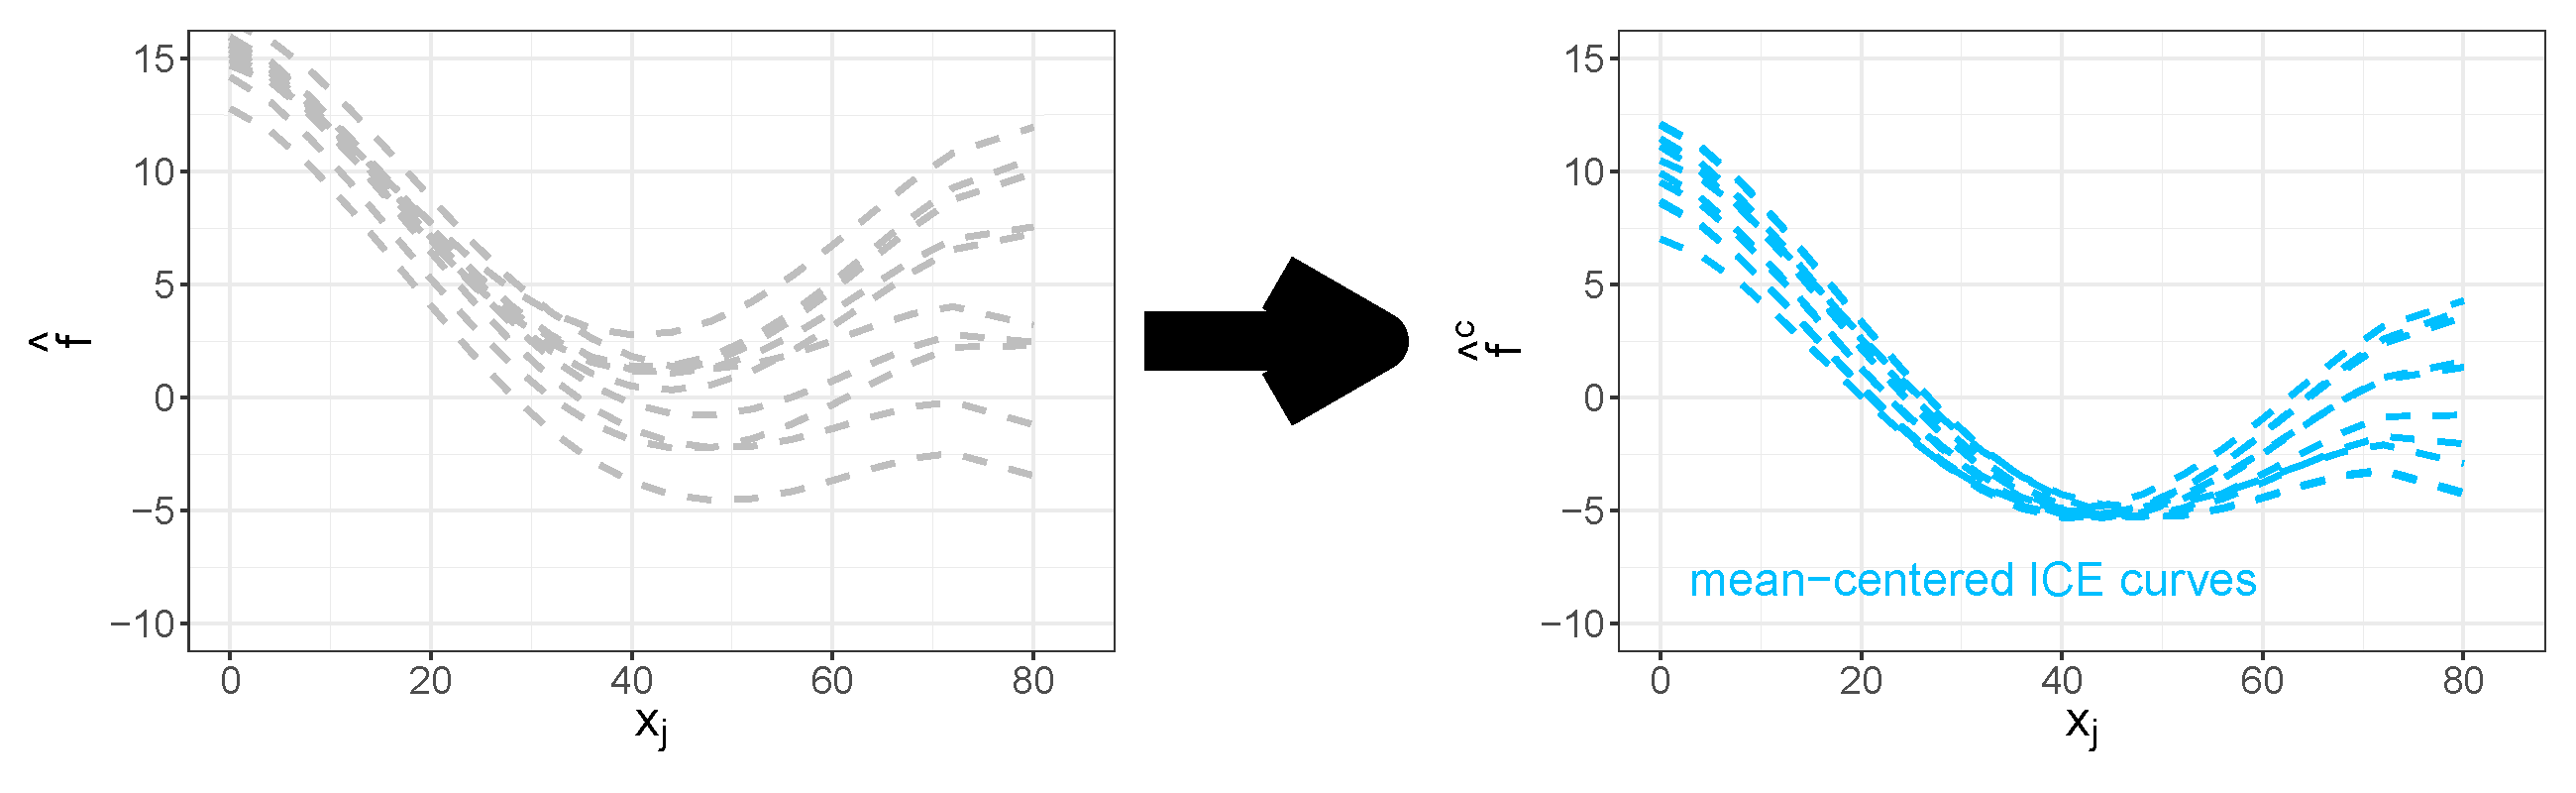
\includegraphics[width = \textwidth]{figure/ice_rep_distance0.png}
        \end{column}
    \end{columns}
    
\end{frame} 




\begin{frame}{GADGET-PD Algorithm}
\begin{itemize}
     \item %Define local effect function $h$ such that we 
     Minimize interactions between feature set $S$ through splits with features in $Z$
     \begin{itemize}
        \item $S$: features to create regional feature effect plots in leaf node (minimize interactions)
        \item $Z$: split features assumed to interact with $S$
     \end{itemize}
     \item REPID is a special case of GADGET-PD where $S = j$ and $Z = -j$
    \item \textbf{Aim:} Recursively partition $\mathcal{X}$ based on features in $Z$ such that (interaction-related) heterogeneity of features in $S$ is minimized, i.e. for each feature $j \in S$, compute:
    %\item Let $h(x_j, \xv_{-j}^{(i)})$ be the $i$-th local feature effect of a feature $\xv_j$ at $x_j \in X_j$
\begin{columns}[T, totalwidth=\textwidth]
    \begin{column}{0.6\textwidth}
   
    \centerline{$\textstyle
    \mathcal{R}_j\left(\mathcal{N}\right) =
    \sum\limits_{\xv \in \mathcal{N}} 
     \sum\limits_{k = 1}^m
     ({\color{cice}\hat f^{c}(\tilde x_j^{(k)}, \xv_{-j})} - {\color{rep}\hat f_{j|\mathcal{N}}^{PD,c} (\tilde x_j^{(k)})})^2
    %\mathcal{L}\left(\xv_j, i\right)
    $}

    \medskip
    
    $\Rightarrow$ Sum risk over all features in $j \in S$: 

    \medskip
    
    \centerline{
    $\textstyle\mathcal{R}(\mathcal{N}) = \sum_{j \in S} \mathcal{R}_j\left(\mathcal{N}\right)$}

    \medskip
    
    $\Rightarrow$ Find the best feature-split combination that minimizes
    
    \medskip
    \centerline{$\textstyle\mathcal{R}\left(\mathcal{N}_{left}\right) + \mathcal{R}\left(\mathcal{N}_{right}\right)$}

    \end{column}
    \begin{column}{0.39\textwidth}
    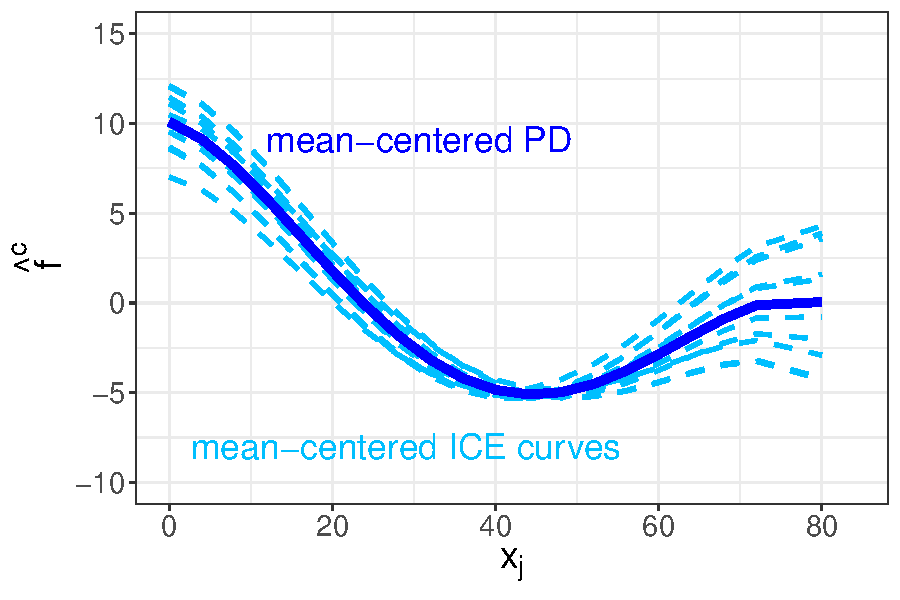
\includegraphics[width = \textwidth]{figure/ice_rep_distance.pdf}
    \end{column}
\end{columns}
  
    $\mathcal{N}_{left} = \{\xv \in \mathcal{N}|x_z \leq t\}$, $\mathcal{N}_{right} = \{\xv \in \mathcal{N}|x_z > t\}$ and split point $t$ for feature $x_z, z \in Z$
    
    % \item $\E[h(x_j, X_{-j})|\mathcal{A}_g]$: expected effect of $\xv_j$ at $x_j$ w.r.t. $X_{-j}$ conditioned on subspace $\mathcal{A}_g \subseteq \mathcal{X}$
    % \begin{itemize}
    %     \item Loss: variance of local effects within $\mathcal{A}_g$ at $x_j$
    %     $$\textstyle\mathcal{L}\left(\mathcal{A}_g, x_j\right) =
    % \sum\limits_{i: \xi \in \mathcal{A}_g}
    %  \left(h(x_j, \mathbf{x}_{-j}^{(i)}) - \E[h (x_j, X_{-j})|\mathcal{A}_g] \right)^2$$
    %  \item Risk: sum over losses of all grid points of $\xv_j$ within $\mathcal{A}_g$
    %  $$\textstyle \mathcal{R}\left(\mathcal{A}_g, \mathbf{x}_j\right) =
    % \sum\limits_{k: k \in \{1,\ldots, m\} \wedge x_j^{(k)} \in \mathcal{A}_g}\mathcal{L}\left(\mathcal{A}_g, x_j^{(k)}\right)$$
    % \end{itemize}
%\end{itemize}
% \begin{eqnarray} 
%     \mathcal{L}\left(\mathcal{A}_g, x_j\right) &=&
%     \sum\limits_{i: \xi \in \mathcal{A}_g}
%      \left(h(x_j, \mathbf{x}_{-j}^{(i)}) - \E[h (x_j, X_{-j})|\mathcal{A}_g] \right)^2
%      \label{eq:loss}
% \end{eqnarray}
% \begin{eqnarray} 
%     \mathcal{R}\left(\mathcal{A}_g, \mathbf{x}_j\right) &=&
%     \sum\limits_{k: k \in \{1,\ldots, m\} \wedge x_j^{(k)} \in \mathcal{A}_g}\mathcal{L}\left(\mathcal{A}_g, x_j^{(k)}\right)
%     \label{eq:risk}
% \end{eqnarray}
%\begin{itemize}
\end{itemize}
%\footnote[frame]{\textbf{Work in progress.}} 
    
\end{frame}




 \begin{frame}{Permutation INTeraction test (PINT)}
 
\begin{itemize}
   \item \textbf{How to choose} $S$ (features to minimize interactions) and $Z$ (split features)?\\
   $\Rightarrow$ In practice, $S = Z = \{1, \dots, p\}$ (but only some features may interact)
   \item \textbf{Goal:} Obtain subset $S$ containing features with significant interactions worth minimizing.
   %Obtain subset $S$ which contains all features that significantly contain interactions (which are worth minimizing their interaction-related heterogeneity) %with each other %w.r.t. a predefined significance level $\alpha$. 
   \item \textbf{Idea:} %Transfer PIMP from loss to predictions (variation of local feature effects)
   %\item 
   %For each feature, compare risk $\mathcal{R}$ with a \textbf{null distribution} 
   Use a permutation test to identify features containing significant interaction-related heterogeneity and ignore spurious interactions (heterogeneity due to correlations / noise)

   $$H_0: \mathcal{R}_j(\Xspace) = 0 \text{ (no interactions present) vs. } H_1: \mathcal{R}_j(\Xspace) > 0$$
   
   %\item With our risk function $\mathcal{R}$ we can \textbf{quantify the heterogeneity of local feature effects} of each feature within the entire feature space. 
   %\item Define a \textbf{null distribution} to determine which \textbf{heterogeneity is actually due to feature interactions} (significant w.r.t. the null distribution) and which heterogeneity is due to e.g. correlations or noise. 
   %\item Permuting only $y$ to \textbf{break the association} between the features and $y$ but \textbf{remain underlying data structure}
   %\item \textbf{Refit} based on the dataset with the permuted $y$ and calculate the risk for each feature \textbf{based on the chosen feature effect method}. 
   %\item \textbf{Repeated $s$ times} to generate the null distribution of risk values for each feature. 
\end{itemize}

\centering
    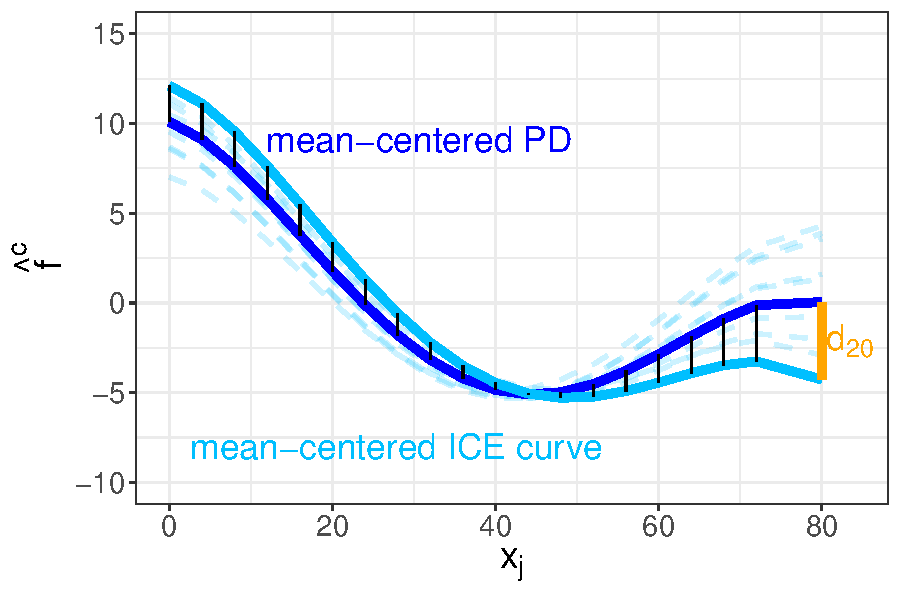
\includegraphics[width = 0.35\textwidth]{figure/ice_rep_distance2.pdf}
 %\footnote[frame]{\textbf{Work in progress.}}
 \end{frame}



\begin{frame}{PINT - Algorithm}

\begin{itemize}
    \item For each repitition $k \in \{1, \ldots, s\}$:
        \begin{itemize}
            \item Permute target $y$ in $\mathcal{D}$ to obtain $\tilde{y}^{k}$ and $\tilde{\mathcal{D}}^{k}$
            \item Refit model on $\tilde{\mathcal{D}}^{k}$ to obtain $\tilde{f}^{k}$
            \item %For each feature $j \in \{1, \ldots, p\}$: 
            Calculate risk $\tilde{\mathcal{R}}_j^{k}(\mathcal{X})$ for each feature $j$ based on $\tilde{\mathcal{D}}^{k}$ and $\tilde{f}^{k}$ (under $H_0$)
        \end{itemize}
    \item For each feature $j \in \{1, \ldots, p\}$:
        \begin{itemize}
            \item Calculate risk {\color{red}$\mathcal{R}_j(\mathcal{X})$} based on $\mathcal{D}$ and $\fh$
            %\item Sort all $\tilde{\mathcal{R}}_j^{k}$ in increasing order
            %\item Set $(1-\alpha)$-quantile $z^{1-\alpha}_j = \tilde{\mathcal{R}}_j^{\lceil (s + 1) (1-\alpha) \rceil}$
            \item Add $j$ to $S$ if and only if {\color{red}$\mathcal{R}_j(\mathcal{X})$} $>$ (1-$\alpha$)-quantile of all $\tilde{\mathcal{R}}_j^1, \dots, \tilde{\mathcal{R}}_j^s$ values
        \end{itemize}
\end{itemize}

\textbf{Example:} Compare {\color{red}$\mathcal{R}_j(\mathcal{X})$} 
with distribution of $\tilde{\mathcal{R}}_j$ values
$\leadsto$ PINT result: $S = \{1, 2\}$
%where after PINT $S = \{1, 2\}$ since {\color{red}$\mathcal{R}_j(\mathcal{X})$} is more extreme then the 95\% quantile
        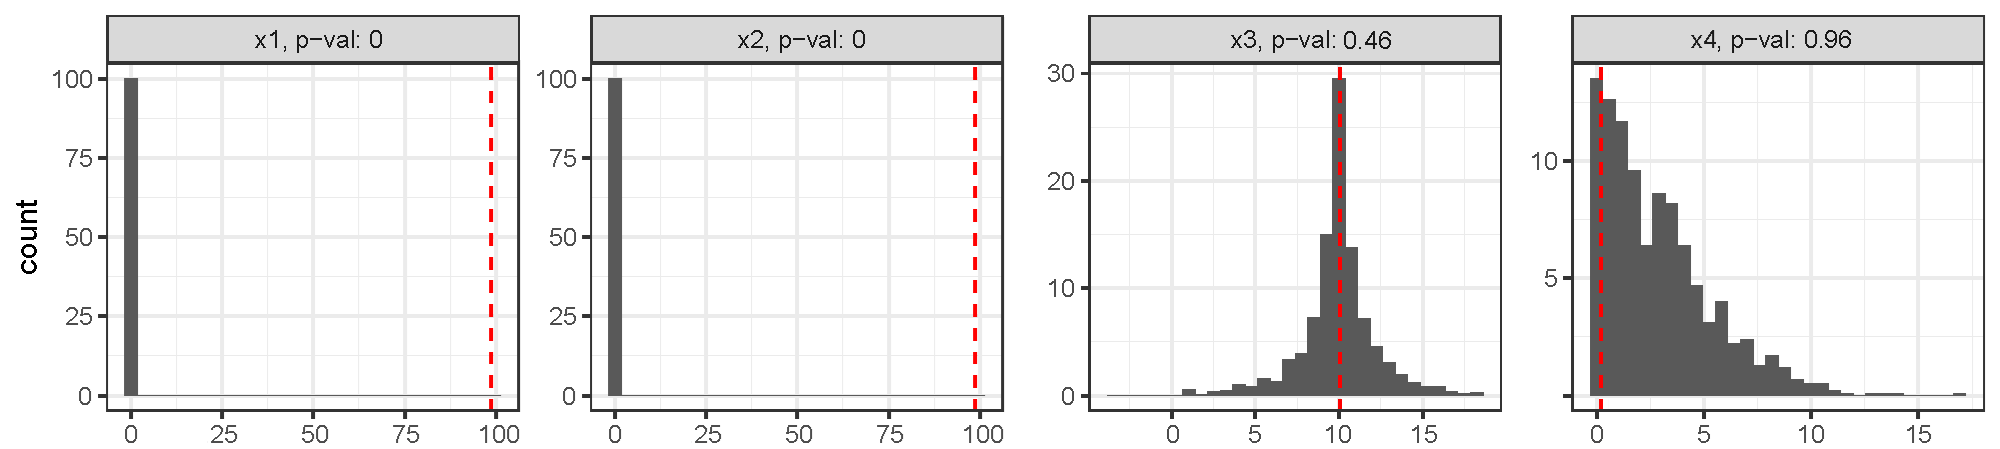
\includegraphics[width=\textwidth]{figure/pint_fake.png}
\end{frame}



\begin{frame}{Conclusion}

\begin{columns}[T, totalwidth = \textwidth]
    \begin{column}{0.53\textwidth}

 \textbf{Summary of Contributions (REPID)}:
 \begin{itemize}
    \item Regional effects in interpretable regions
    \item Additive decomposition of feature effect 
    %\item Prove meaningfulness of objective - only feature interactions between $\xv_j$ and $\xv_{-j}$ minimized %(measures only feature interactions)
    \item Quantify feature interactions 
    \item Outperforms SOTA interaction indices
    %H-Statistics, Greenwell's and Shapley
\end{itemize}

 \textbf{Summary of Contributions (GADGET)}:
 \begin{itemize}
 \item Unique regions for multiple features
 \item Additive decomposition of prediction function%\\
 \item Extension to ALE and Shapley Dependence
% $\Rightarrow$ TODO: Investigate usefulness as ``approximation'' when terminal regions contain interactions
 \item Test to identify significant interactions
\end{itemize}

\textbf{Further Directions}: 

Pruning, GADGET as a predictor, comparing regions across models, efficient implementation, more efficient testing and splitting approach, $\dots$
 
        % \begin{itemize}
        %     \item $f(X) = 3X_1\mathbbm{1}_{X_3>0} - 3X_1\mathbbm{1}_{X_3\leq 0} + X_3 + \epsilon$
        %     \item Features uniformly distributed
        %     \item Left: features independent
        %     \item Right: $X_1$ and $X_3$ highly correlated
        %     \item First split: $\xv_3 \leq 0$ (blue) and $\xv_3 > 0$ (orange)
        % \end{itemize}
    \end{column}
    \begin{column}{0.45\textwidth}
    \centering
    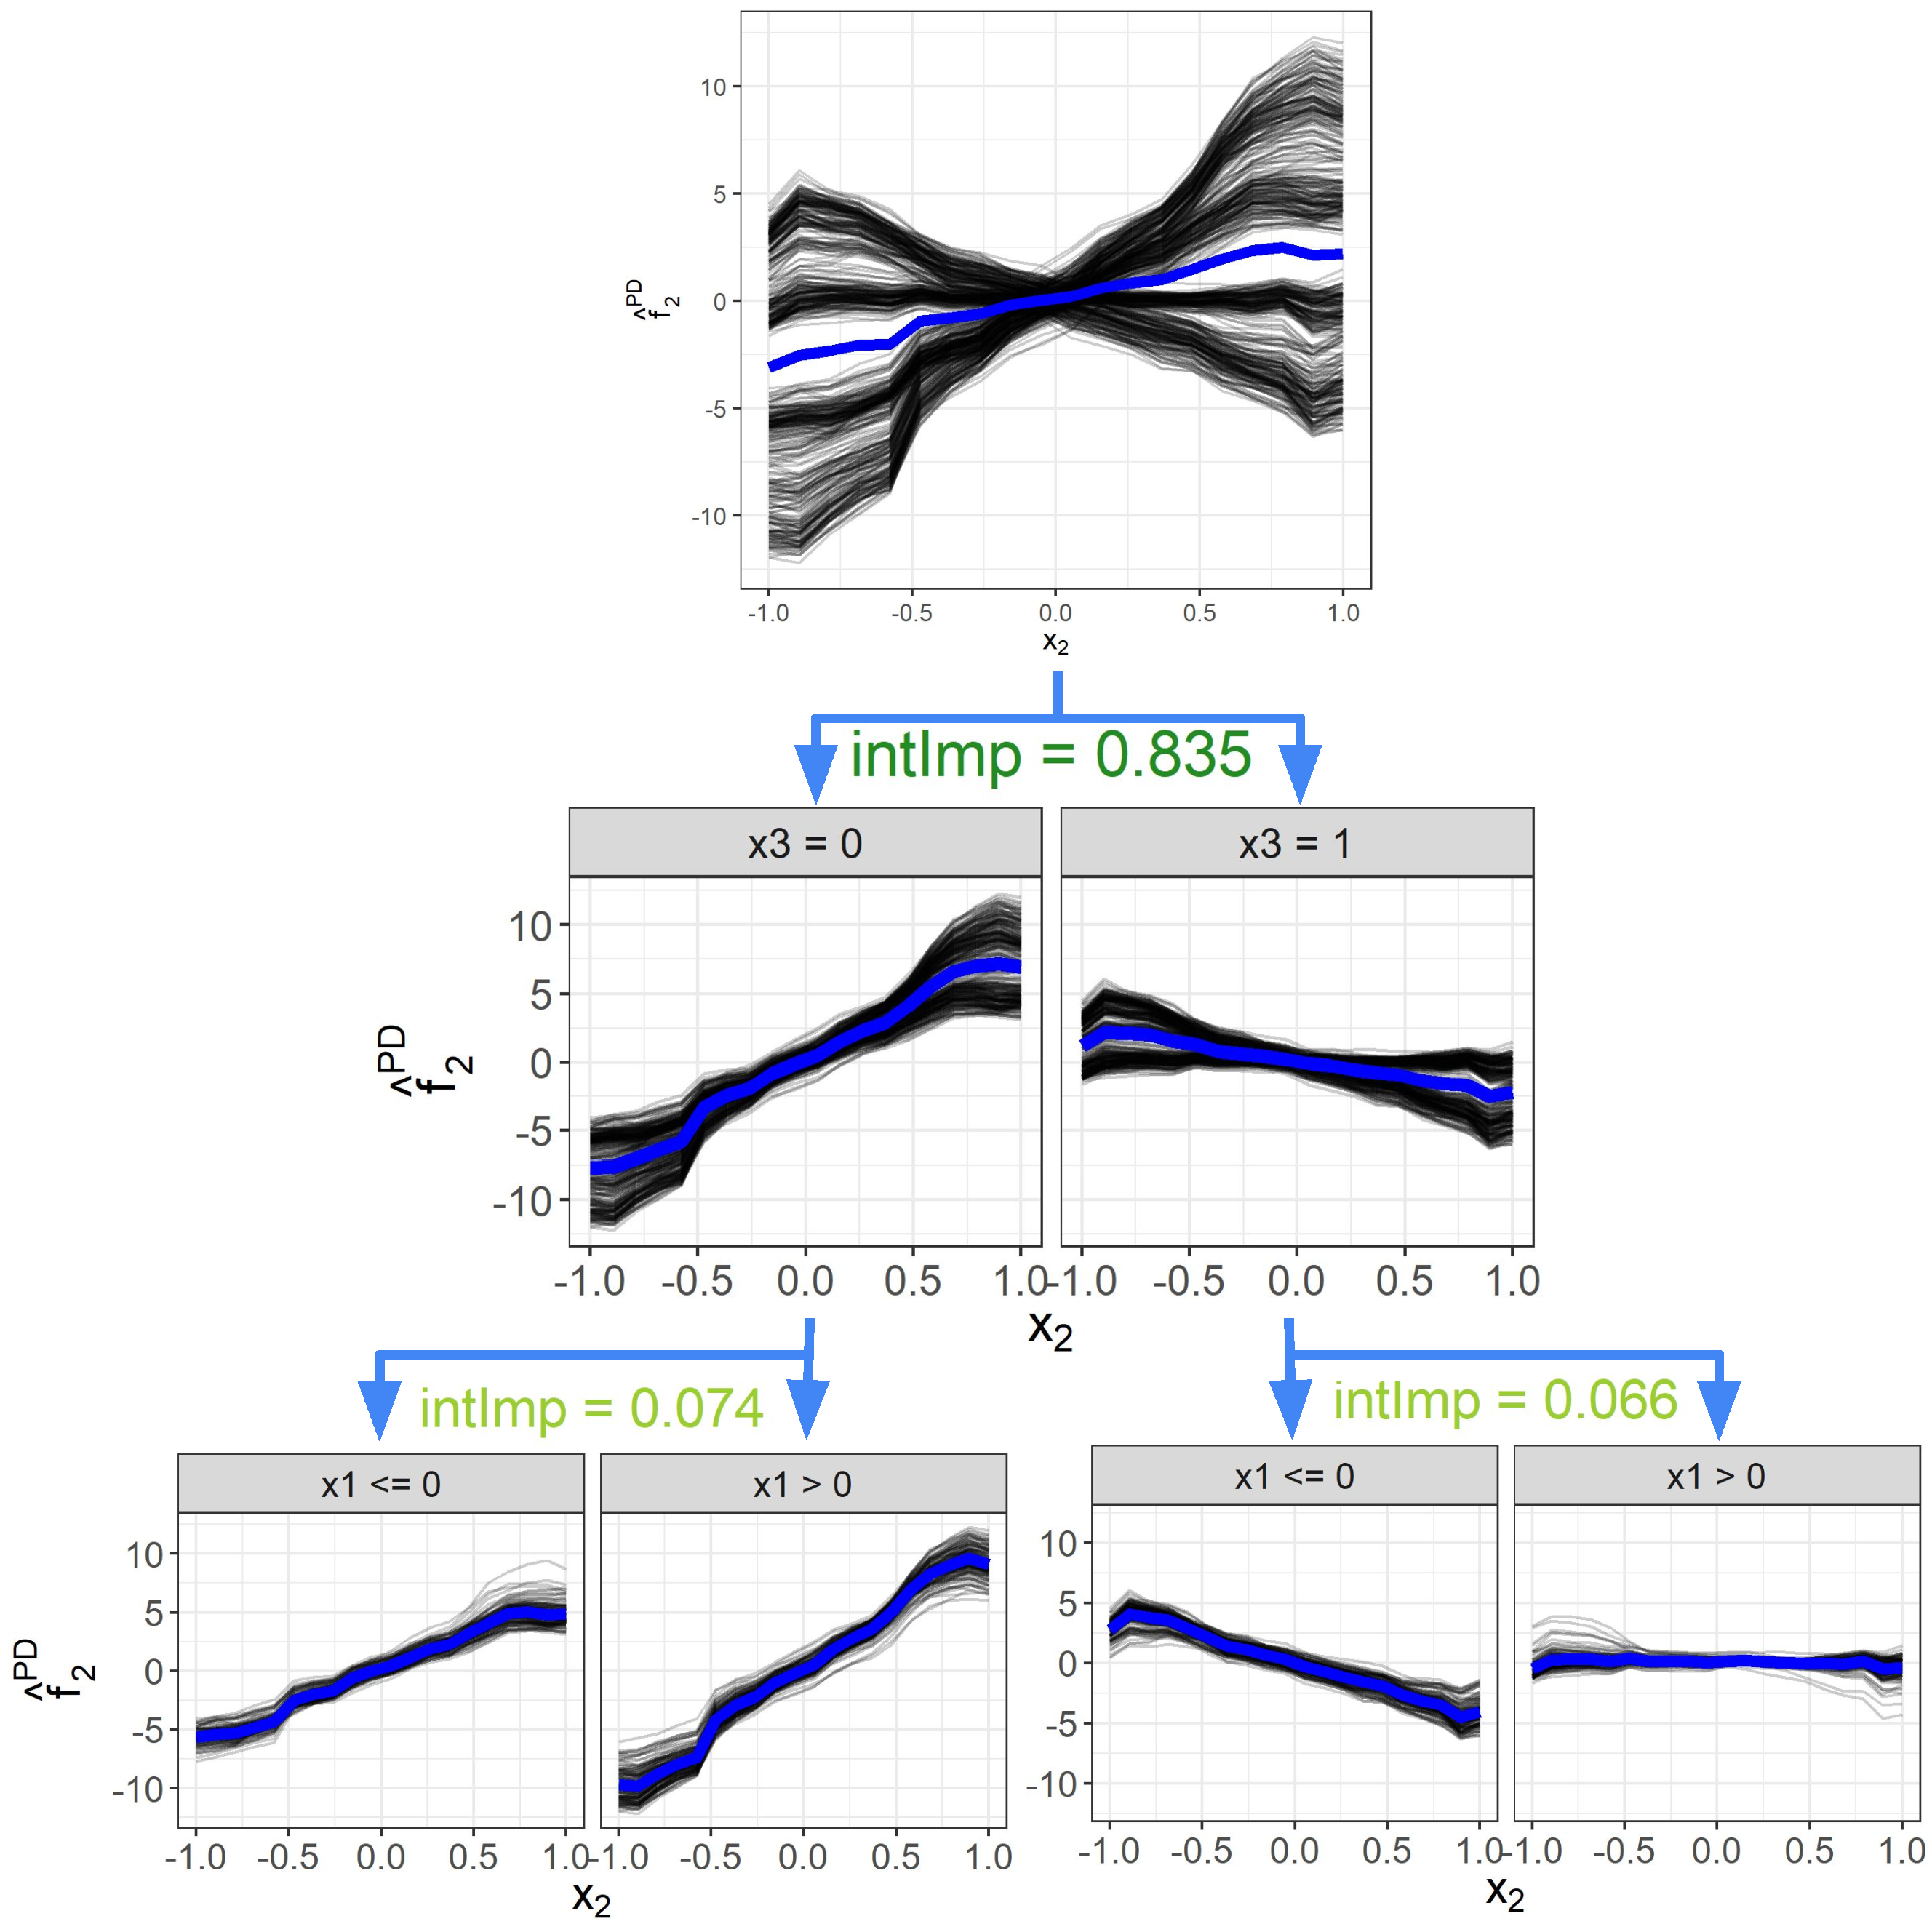
\includegraphics[width=0.95\textwidth]{figure/sim1}
    \vspace{-8pt}
        \begin{columns}[T, totalwidth = \linewidth]
     \footnotesize
            \begin{column}{0.125\linewidth}
            \centering
             $\hat{f}_2^{PD}(X_2)$ %, X_1 > 0 \land X_3 = 0\)\\
         \end{column}
         \begin{column}{0.175\linewidth}
         \centering
             $\approx 8X_2$ %, X_1 > 0 \land X_3 = 0\)\\
         \end{column}
        \begin{column}{0.225\linewidth}
\centering
            $\approx 16X_2$ %, X_1 \leq 0 \land X_3 = 0\)
         \end{column}
        \begin{column}{0.225\linewidth}
        \centering
            $ \approx -8X_2$ %, X_1 \leq 0 \land X_3 \neq 0\)
         \end{column}        
         \begin{column}{0.225\linewidth}
         \centering
             $\approx 0$%, X_1 > 0 \land X_3 \neq 0\)\\
         \end{column}
        \begin{column}{0.025\linewidth}

         \end{column}
     \end{columns}
    \end{column}

\end{columns}
\bigskip
\end{frame}




\endlecture
\end{document}